\chapter{A Numerical Evaluation of the PEM} \label{ch:results}
%
This chapter provides a detailed numerical assessment of the PEM and its variants, with specific emphasis placed on the DG-PEM. Investigations into the sensitivity of the 

\section{Tests for Polynomial Reproducibility}

An investigation was conducted to assess the degree to which polynomial reproducibility was achieved by a given partitioned element methodology. Reproducibility was assessed though the use of an error metric discussed in the following section, herein defined as \textit{interpolation error}.

\subsection*{Interpolation Error}

Consider an arbitrary polytopal element $\Omega \subset \mathbb{R}^d$. Let $u$ denote an arbitrary scalar polynomial field of maximal degree $k$, written in terms of the monomials:
\begin{equation}
        u (\mathbf{X}) = \sum_{|\alpha| \leq k} c_{\alpha} \, \mathbf{X}^{\alpha}.
\end{equation}
The $H^1(\Omega)$ norm of any scalar field $u \in H^1(\Omega)$ will be denoted as
\begin{equation}
        ||u||_{H^1} = \left[ \langle u, \, u \rangle_{H^1} \right]^{1/2},
\end{equation}
where
\begin{equation}
       \langle u,v \rangle_{H^1} = \int_{\Omega} (u \, v + u_{,i} v_{,i}) \, d\Omega
\end{equation}
is the $H^1(\Omega)$ inner product of $u, \,v \in H^1(\Omega)$. Denote $u^h$ as the approximate representation of $u$ over $\Omega$ using the element's shape functions $\left\{ \varphi_A \right\}_{A=1}^{N^\Omega_V}$:
\begin{equation}
        u^h (\mathbf{X}) = \sum_{A = 1}^{N^{\Omega}_V} \varphi_A (\mathbf{X}) \, u(\mathbf{X}_A).
\end{equation}

The space of all polynomials of maximal degree $k$ is denoted as $P^k (\Omega)$. We will confine our attention to the sub-space $\bar{P}^k (\Omega) \subset P^k (\Omega)$ containing only those polynomials with unit $H^1 (\Omega)$ norm:
\begin{equation}
        \bar{P}^k (\Omega) = \{ u : u \in P^k (\Omega), ||u||_{H^1} = 1 \}.
\end{equation}

The \textit{interpolation error} $E_k (\Omega)$ on the element $\Omega$ for the polynomials of maximal degree $k$ is defined as
\begin{equation}
        E_k (\Omega) \equiv \max_{u \in \bar{P}^k (\Omega)} || u(\mathbf{X}) - u^h(\mathbf{X}) ||_{H^1} = \max_{u \in P^k (\Omega)} \frac{|| u(\mathbf{X}) - u^h(\mathbf{X}) ||_{H^1}}{|| u(\mathbf{X}) ||_{H^1}}.
\end{equation}
In the computation of this error measure, we must determine the polynomial coeffients $c_\alpha$ of $u \in \bar{P}^k (\Omega)$ which yield the maximal error. Denote $e_\alpha$ as the error in the approximation of the monomial $\mathbf{X}^\alpha$:
\begin{equation}
        e_\alpha = \mathbf{X}^{\alpha} - \sum_{A = 1}^{N^{\Omega}_V} \varphi_A (\mathbf{X}) \, \mathbf{X}_A^{\alpha}.
\end{equation}
Consequently,
\begin{equation}
        \left[ E_k (\Omega) \right]^2 = \max_{c_\gamma} \sum_{|\alpha| \leq k} \sum_{|\beta| \leq k} c_{\alpha} c_{\beta} \langle e_\alpha, e_\beta \rangle_{H^1},
\end{equation}
subject to the constraint
\begin{equation}
        g(c_\gamma) = 1 - \sum_{|\alpha| \leq k} \sum_{|\beta| \leq k} c_{\alpha} c_{\beta} \langle \mathbf{X}^\alpha, \mathbf{X}^\beta \rangle_{H^1} = 0.
\end{equation}
Using the method of Lagrange multipliers, we may rewrite the above constrained optimization problem as
\begin{equation}
        \left[ E_k (\Omega) \right]^2 = \max_{c_\gamma, \lambda} \Lambda (c_\gamma,\lambda),
\end{equation}
where $\Lambda (c_\gamma,\lambda)$ is the Lagrangian:
\begin{equation}
        \Lambda (c_\gamma, \lambda) = \max_{c_\gamma} \sum_{|\alpha| \leq  k} \sum_{|\beta| \leq k} c_{\alpha} c_{\beta} \langle e_\alpha, e_\beta \rangle_{H^1} + \lambda g(c_\gamma).
\end{equation}
Observe that
\begin{equation}
        \frac{\partial}{\partial \lambda} \Lambda (c_\gamma, \lambda) = g(c_\gamma) = 0,
\end{equation}
and
\begin{equation}
        \frac{\partial}{\partial c_\gamma} \Lambda (c_\gamma, \lambda) = \sum_{|\alpha| \leq k} \sum_{|\beta| \leq k} \frac{\partial}{\partial c_\gamma} (c_{\alpha} c_{\beta}) \langle e_\alpha, e_\beta \rangle_{H^1} + \lambda \frac{\partial}{\partial c_\gamma} g(c_\gamma) = 0.
\end{equation}
This yields
\begin{equation}
        \sum_{|\alpha| \leq k} c_{\alpha} \left[ \langle e_\alpha, e_\gamma \rangle_{H^1} - \lambda \langle \mathbf{X}^\alpha, \mathbf{X}^\gamma \rangle_{H^1} \right] = 0 \quad \forall |\gamma| \leq k,
\end{equation}
or, in matrix-vector notation:
\begin{equation}
        (\mathbf{A} - \lambda \mathbf{B}) \mathbf{c} = \mathbf{0},
\end{equation}
which corresponds to a generalized eigenvalue problem, where
\begin{equation}
        A_{\alpha \beta} = \langle e_\alpha, e_\beta \rangle_{H^1}, \qquad B_{\alpha \beta} = \langle \mathbf{X}^\alpha, \mathbf{X}^\beta \rangle_{H^1},
\end{equation}
are both real, symmetric matrices. Since $\mathbf{B}$ is positive-definite, we determine that it is invertible, and therefore we may solve the equivalent eigenvalue problem
\begin{equation}
        (\mathbf{B}^{-1} \mathbf{A} - \lambda \mathbf{1}) \mathbf{c} = \mathbf{0}.
\end{equation}
The square root of the maximum eigenvalue $\lambda_{\max}$ of $\mathbf{B}^{-1} \mathbf{A}$ yields the interpolation error $E_k (\Omega) = \sqrt{\lambda_{\max}}$. This can be seen more directly if we view $\left[ E_k (\Omega) \right]^2$ to be the generalized Rayleigh quotient of $\mathbf{A}$ and $\mathbf{B}$:
\begin{equation}
        E_k (\Omega) = \max_{\mathbf{c}} \sqrt{\frac{\mathbf{c}^T \mathbf{A} \mathbf{c}}{\mathbf{c}^T \mathbf{B} \mathbf{c}}} = \sqrt{\lambda_{\max}}.
\end{equation}
For simplicity in the numerical computation of $E_k (\Omega)$, we assume that the entries of $\mathbf{A}$ and $\mathbf{B}$ will be computed approximately using the element's quadrature rules, i.e.
\begin{equation}
        \langle e_\alpha, e_\beta \rangle_{H^1} \approx \sum_{q=1}^{N^{\Omega}_{qp}} w_q (e_{\alpha}^{q} e_{\beta}^{q} + e_{\alpha,i}^{q} e_{\beta,i}^{q})
\end{equation}
\begin{equation}
        \langle \mathbf{X}^\alpha, \mathbf{X}^\beta \rangle_{H^1} \approx \sum_{q=1}^{N^{\Omega}_{qp}} w_q (\mathbf{X}^{\alpha}_{q} \mathbf{X}^{\beta}_{q} + \mathbf{X}^{\alpha}_{q,i} \mathbf{X}^{\beta}_{q,i})
\end{equation}
where
\begin{equation}
        e_{\alpha}^{q} = \mathbf{X}^{\alpha}_{q} - \sum_{A = 1}^{N^{\Omega}_V} \varphi_A (\mathbf{X}_{q}) \, \mathbf{X}_A^{\alpha}, \qquad e_{\alpha,i}^{q} = \mathbf{X}^{\alpha}_{q,i} - \sum_{A = 1}^{N^{\Omega}_V} \varphi_{A,i} (\mathbf{X}_{q}) \, \mathbf{X}_A^{\alpha}.
\end{equation}

If a given element is capable of reproducing all polynomials up to degree $k$, then clearly $E_k(\Omega) = 0$. This property will be used to verify that the shape function approximations obtained via a particular formulation of the PEM satisfy the requirements of polynomial reproducibility.

\subsection*{Polynomial Reproducibility of PEM Elements}

Through a series of numerical experiments, we confirm that both the CG-PEM and the DG-PEM satisfy the requirements of polynomial reproducibility. Particular attention is paid to low-order PEM elements (i.e. $k=1$), where satisfaction of the condition $E_1 (\Omega) = 0$ is sufficient to demonstrate reproducibility for a given element $\Omega$.

Consider the arbitrary polygonal element and its corresponding edge-based partition illustrated in Figure \ref{fig:reproducing_element_shape}. The harmonic shape functions defined on this partitioned element were approximated using the CG-PEM and the DG-PEM. Unless otherwise noted, the NIPG version of the DG-PEM (with $\epsilon = +1$) was utilized throughout.

\begin{figure}[!h]
  \centering
  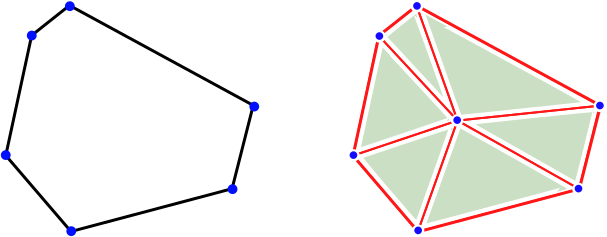
\includegraphics[width=3.5in]{figures/reproducing_element_shape.pdf}  \caption{A representative polygonal element and its corresponding edge-based partition.}
  \label{fig:reproducing_element_shape}
\end{figure}

For the partitioned element under consideration, the interpolation error of order $k=1$ for the CG-PEM was computed as $E_1 (\Omega) = 2.5465 \times 10^{-16}$ (on the order of machine precision). For the DG-PEM, the interpolation error was observed to be dependent upon the accuracy of the computations performed in solving (\ref{eq:dgpem_linear_system}). The log of $\kappa(\mathbf{J})$ provides a useful indicator of the number of digits of precision lost in computing $\mathbf{J}^{-1}$. This loss of precision is reflected by a corresponding increase in the interpolation error measure. Table \ref{tab:interpolation_error_and_condJ_k1} illustrates the connection between $E_1 (\Omega)$ and $\kappa(\mathbf{J})$ for various DG-PEM penalty parameter values. 

\begin{table}
\centering
\begin{subtable}{1.0\textwidth}
\centering
\begin{tabular}{| c || c | c | c | c |}
    \hline
DG-PEM & $\alpha_{0\gamma} = 10^{-3}$ & $\alpha_{0\gamma} = 10^{0}$ & $\alpha_{0\gamma} = 10^{3}$ & $\alpha_{0\gamma} = 10^{6}$ \\ \hline \hline
$\alpha_{1\gamma} = 0.0$	& 1.66E-013 & 7.48E-016 & 4.70E-014 & 1.79E-010 \\ \hline
$\alpha_{1\gamma} = 10^{0}$ & 1.65E-013 & 9.67E-016 & 8.73E-015 & 2.51E-011 \\ \hline
$\alpha_{1\gamma} = 10^{3}$ & 1.01E-012 & 2.66E-013 & 1.36E-015 & 4.49E-014 \\ \hline
$\alpha_{1\gamma} = 10^{6}$ & 1.13E-009 & 3.13E-010 & 7.10E-013 & 9.03E-016 \\
    \hline
    \end{tabular}
    \caption{Interpolation error: $E_1 (\Omega)$}
    \label{tab:interpolation_error_k1}
\end{subtable}% <---- don't forget this %
\\
\begin{subtable}{1.0\textwidth}
\centering
\begin{tabular}{| c || c | c | c | c |}
    \hline
DG-PEM & $\alpha_{0\gamma} = 10^{-3}$	&	$\alpha_{0\gamma} = 10^{0}$	&	$\alpha_{0\gamma} = 10^{3}$	&	$\alpha_{0\gamma} = 10^{6}$ \\ \hline \hline
$\alpha_{1\gamma} = 0.0$	&	5.44E+002 & 4.07E+000 & 5.94E+003 & 5.96E+006 \\ \hline
$\alpha_{1\gamma} = 10^{0}$	&	4.96E+003 & 2.01E+001 & 9.33E+002 & 9.29E+005 \\ \hline
$\alpha_{1\gamma} = 10^{3}$	&	1.58E+007 & 2.50E+004 & 6.96E+001 & 1.11E+003 \\ \hline
$\alpha_{1\gamma} = 10^{6}$	&	2.37E+010 & 2.50E+007 & 6.86E+004 & 6.98E+001 \\
    \hline
    \end{tabular}
    \caption{DG-PEM linear system conditioning: $\kappa(\mathbf{J})$}
    \label{tab:condJ_k1}
\end{subtable}

\caption{Computed values of $E_1 (\Omega)$ and $\kappa(\mathbf{J})$ for the element in Figure \ref{fig:reproducing_element_shape}, using various DG-PEM penalty parameter settings.}
\label{tab:interpolation_error_and_condJ_k1}
\end{table}

The results in table \ref{tab:interpolation_error_and_condJ_k1} confirm that $\mathbf{J}$ will become poorly conditioned if either of the two penalty parameters $\alpha_{0\gamma}$ or $\alpha_{1\gamma}$ are sufficiently large. This is true regardless of how the DG polynomial bases are specified within each geometric entity. Under certain circumstances, $\mathbf{J}$ will remain well-conditioned if both $\alpha_{0\gamma}$ and $\alpha_{1\gamma}$ are kept roughly proportional to one another, for all values of $\alpha_{0\gamma}, \, \alpha_{1\gamma} > 0$. If $\alpha_{0\gamma}$ and $\alpha_{1\gamma}$ are increased proportionally to one another, one recovers the behavior of the pure penalty DG-PEM in (\ref{eq:pure_penalty}).

It is remarked that other factors which impact with condition number of $\mathbf{J}$ may have detrimental effects on the accuracy of the element's interpolation error. Specifically, consider the case where the element in Figure \ref{fig:reproducing_element_shape} is scaled anisotropically by a factor of $0.01$ in the vertical direction, yielding a comparatively thin element with an aspect ratio of 100:1. For this element, the interpolation error using the CG-PEM increases only slightly, to $E_1 (\Omega) = 6.9817 \times 10^{-15}$. The corresponding values of $E_1 (\Omega)$ and $\kappa(\mathbf{J})$ for the DG-PEM are presented in table \ref{tab:thin_interpolation_error_and_condJ_k1}.

\begin{table}
\centering
\begin{subtable}{1.0\textwidth}
\centering
\begin{tabular}{| c || c | c | c | c |}
    \hline
DG-PEM & $\alpha_{0\gamma} = 10^{-3}$ & $\alpha_{0\gamma} = 10^{0}$ & $\alpha_{0\gamma} = 10^{3}$ & $\alpha_{0\gamma} = 10^{6}$ \\ \hline \hline
$\alpha_{1\gamma} = 0.0$	& 3.02E-014 & 9.01E-015 & 5.22E-013 & 1.59E-009 \\ \hline
$\alpha_{1\gamma} = 10^{0}$ & 3.99E-014 & 1.37E-014 & 2.02E-013 & 3.12E-012 \\ \hline
$\alpha_{1\gamma} = 10^{3}$ & 2.44E-011 & 6.48E-012 & 1.89E-012 & 3.34E-013 \\ \hline
$\alpha_{1\gamma} = 10^{6}$ & 1.52E-007 & 4.97E-008 & 1.85E-009 & 3.69E-012 \\
    \hline
    \end{tabular}
    \caption{Interpolation error: $E_1 (\Omega)$}
    \label{tab:thin_interpolation_error_k1}
\end{subtable}% <---- don't forget this %
\\
\begin{subtable}{1.0\textwidth}
\centering
\begin{tabular}{| c || c | c | c | c |}
    \hline
DG-PEM & $\alpha_{0\gamma} = 10^{-3}$	&	$\alpha_{0\gamma} = 10^{0}$	&	$\alpha_{0\gamma} = 10^{3}$	&	$\alpha_{0\gamma} = 10^{6}$ \\ \hline \hline
$\alpha_{1\gamma} = 0.0$	& 9.07E+003 & 1.39E+002 & 1.14E+005 & 1.33E+008 \\ \hline
$\alpha_{1\gamma} = 10^{0}$	& 3.52E+005 & 1.75E+003 & 1.97E+004 & 3.67E+005 \\ \hline
$\alpha_{1\gamma} = 10^{3}$	& 1.17E+009 & 2.46E+006 & 2.61E+005 & 2.32E+004 \\ \hline
$\alpha_{1\gamma} = 10^{6}$	& 1.77E+012 & 2.45E+009 & 2.52E+008 & 3.07E+005 \\
    \hline
    \end{tabular}
    \caption{DG-PEM linear system conditioning: $\kappa(\mathbf{J})$}
    \label{tab:thin_condJ_k1}
\end{subtable}

\caption{Computed values of $E_1 (\Omega)$ and $\kappa(\mathbf{J})$ for a comparatively thin element with an aspect ratio of 100:1, using various DG-PEM penalty parameter settings.}
\label{tab:thin_interpolation_error_and_condJ_k1}
\end{table}

Clearly, a careful selection of $\alpha_{0\gamma}$ and $\alpha_{1\gamma}$ is warranted for the sake of minimizing the resulting interpolation error. For general 2D applications in which an edge-based partitioning scheme is employed, it is suggested that the parameter values be chosen such that $\alpha_{0\gamma} = 10.0$ and $\alpha_{1\gamma} = 0.0$. However, it is recommended that a more thorough investigation be conducted to determine more optimal parameters settings for other element types.

\section{Finite Element Patch Tests}

In this section we investigate the behavior of PEM elements in the context of the classical patch test introduced by Irons in the Appendix of \cite{Irons:65}, whose passage is argued in \cite{Simo&Taylor:86} to be a necessary and sufficient condition for convergence. This claim has been disputed, namely by Stummel in \cite{Stummel:80}. Nonetheless, it serves as a useful indicator for the expected convergence properties of conforming finite elements. Two tests will be considered: the linear and quadratic patch tests, as depicted in figure \ref{fig:polygonal_patches}.

\begin{figure}[!h]
    \centering
    \begin{subfigure}[b]{0.49\linewidth}
            \centering
            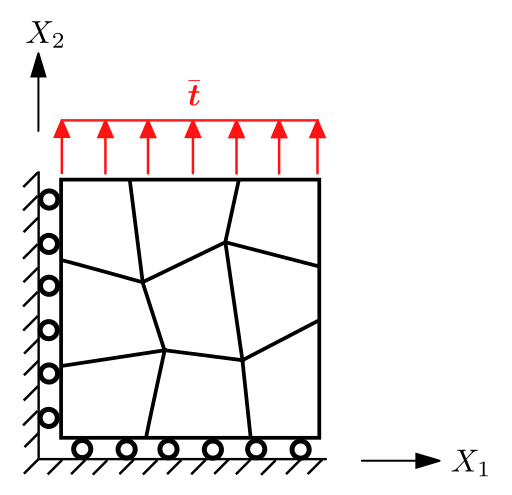
\includegraphics[width=2.5in]{figures/linear_patch_test.pdf}
    			\caption{linear patch test \label{fig:linear_patch_test}}
    \end{subfigure}
	\begin{subfigure}[b]{0.49\linewidth}
            \centering
            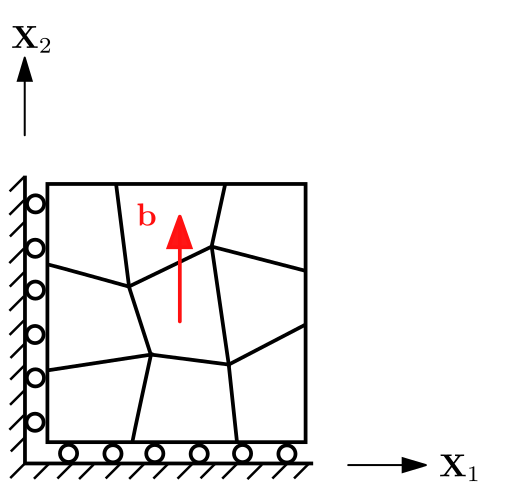
\includegraphics[width=2.5in]{figures/quadratic_patch_test.pdf}
    			\caption{quadratic patch test \label{fig:quadratic_patch_test}}
    \end{subfigure}
    \caption{Depiction of simple patch tests for (\subref{fig:linear_patch_test}) linear and (\subref{fig:quadratic_patch_test}) quadratic elements.}
    \label{fig:polygonal_patches}
\end{figure}

The linear patch test consists of a square patch of elements with dimensions $L \times L$. The normal components of displacement on the $-X_1$ and $-X_2$ faces of the patch are constrained such that
\begin{equation}
	u_1 (X_2 = 0) = 0, \quad u_2 (X_1 = 0) = 0.
\end{equation}
A constant vertical traction $\bar{\mathbf{t}} = (0, \, T)$ is prescribed on the $+X_2$ face of the patch. For a linear elastic body under plane strain conditions, an exact solution for the in-plane displacement and stress fields is easily obtained:
\begin{equation}
	u_1 (\mathbf{X}) = - \frac{\nu}{2 \mu} T X_1, \quad u_2 (\mathbf{X}) = \frac{(1-\nu)}{2 \mu} T X_2,
\end{equation}
\begin{equation}
	\sigma_{11} (\mathbf{X}) = \sigma_{12} (\mathbf{X}) = 0, \quad \sigma_{22} (\mathbf{X}) = T.
\end{equation}

For the quadratic patch test, we will consider a similarly constrained square patch as for the linear patch test. A constant body force $\mathbf{b} = (b_1, \, b_2)$ acts uniformly over the patch. Additionally, linearly varying tractions are applied to the unconstrained faces of the patch:
\begin{equation}
	\bar{t}_1 (X_1 = L) = - \frac{\lambda}{\lambda + 2 \mu} b_2 X_2, \quad \bar{t}_2 (X_1 = L) = 0,
\end{equation}
\begin{equation}
	\bar{t}_2 (X_2 = L) = - \frac{\lambda}{\lambda + 2 \mu} b_1 X_2, \quad \bar{t}_1 (X_2 = L) = 0.
\end{equation}
For a linear elastic material under plane strain conditions, an exact solution may be obtained of the form:
\begin{equation}
	u_1 (\mathbf{X}) = \frac{b_1}{2 (\lambda + 2 \mu)} (L - X_1) X_1 + \frac{\nu (b_1 - b_2)}{2 \mu} L X_1,
\end{equation}
\begin{equation}
	u_2 (\mathbf{X}) = \frac{b_2}{2 (\lambda + 2 \mu)} (L - X_2) X_2 + \frac{\nu (b_2 - b_1)}{2 \mu} L X_2,
\end{equation}
\begin{equation}
	\sigma_{11} (\mathbf{X}) = b_1 (L - X_1) + \frac{\lambda}{\lambda + 2 \mu} b_2 X_2,
\end{equation}
\begin{equation}
	\sigma_{22} (\mathbf{X}) = b_2 (L -  X_2) + \frac{\lambda}{\lambda + 2 \mu} b_1 X_1,
\end{equation}
\begin{equation}
	\sigma_{12} (\mathbf{X}) = 0.
\end{equation}
A simplistic case involving only a constant body force and no boundary tractions occurs when $\nu = 0$ and $b_1 = 0$:
\begin{equation}
	u_1 (\mathbf{X}) = 0, \quad u_2 (\mathbf{X}) = \frac{b_2}{2 (\lambda + 2 \mu)} (L - X_2) X_2,
\end{equation}
\begin{equation}
	\sigma_{11} (\mathbf{X}) = \sigma_{12} (\mathbf{X}) = 0, \quad \sigma_{22} (\mathbf{X}) = b_2 (L -  X_2).
\end{equation}

Patch test errors were measured in terms of the normalized $L^2 (\Omega)$ error metrics for displacement and stress:
\begin{equation}
	\frac{||\mathbf{u}^h - \mathbf{u}||}{||\mathbf{u}||} = \sqrt{\frac{\int_{\mathcal{B}_0} (\mathbf{u}^h - \mathbf{u}) \cdot (\mathbf{u}^h - \mathbf{u}) \, dV}{\int_{\mathcal{B}_0} \mathbf{u} \cdot \mathbf{u} \, dV}},
\end{equation}
\begin{equation}
	\frac{||\boldsymbol{\sigma}^h - \boldsymbol{\sigma}||}{||\boldsymbol{\sigma}||} = \sqrt{\frac{\int_{\mathcal{B}_0} (\boldsymbol{\sigma}^h - \boldsymbol{\sigma}) \colon (\boldsymbol{\sigma}^h - \boldsymbol{\sigma}) \, dV}{\int_{\mathcal{B}_0} \boldsymbol{\sigma} \colon \boldsymbol{\sigma} \, dV}},
\end{equation}
where $\mathbf{u}$ and $\boldsymbol{\sigma}$ denote the exact solutions for the displacement and stress fields, respectively.

\subsection*{Linear Patch Tests}

The two meshes depicted in Figure \ref{fig:patch_test_meshes} are considered. The PEM was used on the polygonal mesh, whereas the FEM with standard 4-nodes isoparametric elements was used on the quadrilateral mesh.

\begin{figure}[!h]
    \centering
    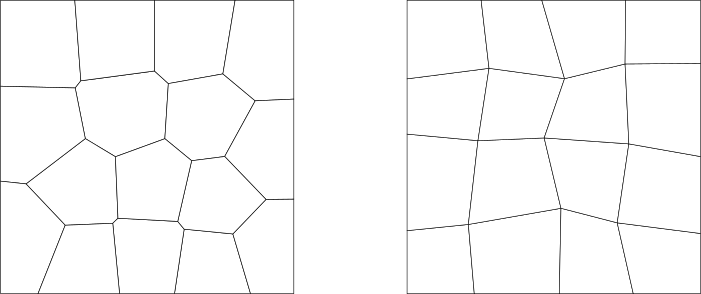
\includegraphics[width=4.0in]{figures/patch_test_meshes.pdf}
    	\caption{Meshes used for the linear patch test: (left) polygonal mesh, (right) distorted quadrilateral mesh.}
    \label{fig:patch_test_meshes}
\end{figure}

Linear patch test errors for the FEM, CG-PEM, and DG-PEM were explored. Both the CG-PEM and DG-PEM utilized an edge-based partitioning scheme and composite mid-point quadrature rules for each element. Unless otherwise noted, the parameters for the DG-PEM were selected as $\epsilon = +1$, $\alpha_{0\gamma} = 10.0$, and $\alpha_{1\gamma} = 0.0$. Further, the DG-PEM was tested both with and without using the gradient correction scheme presented in \cite{Talischi:15}. These corrections were applied to the test function gradients alone (yielding a ``nonsymmetric correction'' scheme), or to both the trial and test function gradients (yielding a ``symmetric correction'' scheme). The results of these tests may be found in table \ref{tab:linear_patch_test}.

\begin{table}[!ht]
  \begin{center}
    \begin{tabular}{| c || c | c |}
    \hline
           & $||\mathbf{u}^h - \mathbf{u}|| / ||\mathbf{u}||$ & $||\boldsymbol{\sigma}^h - \boldsymbol{\sigma}|| / ||\boldsymbol{\sigma}||$ \\ \hline \hline
    FEM (4-node quadrilaterals) & 5.1568E-015 & 7.7395E-016 \\ \hline
    CG-PEM (no gradient correction) & 5.9125E-012 & 5.1637E-012 \\ \hline
    DG-PEM (no gradient correction) & 2.7721E-005 & 3.0904E-004 \\ \hline
    DG-PEM (symmetric correction) & 6.2750E-012 & 5.3521E-012 \\ \hline
    DG-PEM (nonsymmetric correction) & 6.2673E-012 & 5.3494E-012 \\
    \hline
    \end{tabular}
    \caption{Linear patch test results comparison for FEM, CG-PEM, and DG-PEM.}
    \vspace{-5pt}
    \label{tab:linear_patch_test}
    \vspace{-25pt}
  \end{center}
\end{table}

The classical FEM produces errors on the order of machine precision. The CG-PEM produces results that are only slightly less accurate. Interestingly, the errors for the CG-PEM are unaffected by the use (or disuse) of a gradient correction scheme. In contrast, the DG-PEM produces noticeable errors if no gradient correction scheme is employed. Using either of the symmetric or nonsymmetric gradient correction schemes with the DG-PEM yields comparable accuracy to the CG-PEM.

These observations help to illuminate an important point regarding a consistent integration of the weak form. Consider the consistency equations in (\ref{eq:consistency}). It is remarked that any continuous field $\varphi_a \in C^0 (\Omega_e)$ integrated exactly in (\ref{eq:consistency}) will lead to direct satisfaction of quadrature consistency. Such is the case for the CG-PEM under the present circumstances. However, if $\varphi_a$ is not a continuous field, neither (\ref{eq:consistency}) nor quadrature consistency will not not be satisfied, in general. Such is the case for the DG-PEM, even when exact integration is used. The consequence is violation of patch tests. This can be mitigated through the use of a gradient correction scheme, or alternatively through an appropriate selection of the DG-PEM parameters. Specifically, in the limit as $\alpha_{0\gamma} \rightarrow \infty$, the DG-PEM reduces to the CG-PEM, and the resulting patch test errors can be eliminated. Table \ref{tab:linear_patch_test_parameter_study} demonstrates this behavior for increasing values of $\alpha_{0\gamma}$, in the absence of a gradient correction scheme.

\begin{table}[!ht]
  \begin{center}
    \begin{tabular}{| c || c | c | c | c | c |}
    \hline
    DG-PEM & $\alpha_{0\gamma} = 10^{-6}$ & $\alpha_{0\gamma} = 10^{-3}$ & $\alpha_{0\gamma} = 10^{0}$ & $\alpha_{0\gamma} = 10^{3}$ & $\alpha_{0\gamma} = 10^{6}$ \\ \hline \hline
    	$\alpha_{1\gamma} = 0.0$ & 2.8433E-009 & 2.8152E-006 & 3.3114E-004 & 4.8035E-006 & 4.8278E-009 \\ \hline
    $\alpha_{1\gamma} = 10^{-3}$ & 2.8505E-009 & 2.8224E-006 & 3.2288E-004 & 4.9805E-006 & 5.0082E-009 \\ \hline
    $\alpha_{1\gamma} = 10^{0}$ & 3.4853E-009 & 3.4604E-006 & 2.4827E-003 &  7.4284E-004 & 8.6376E-007 \\ \hline
    $\alpha_{1\gamma} = 10^{3}$ & 3.5460E-009 & 3.5450E-006 & 3.0047E-003 & 1.3898E-002 & 7.4705E-004 \\ \hline
    $\alpha_{1\gamma} = 10^{6}$ & 3.5457E-009 & 3.5456E-006 & 3.0054E-003 & 1.4604E-002 & 1.3953E-002 \\
    \hline
    \end{tabular}
    \caption{Computed values of $||\boldsymbol{\sigma}^h - \boldsymbol{\sigma}|| / ||\boldsymbol{\sigma}||$ for the DG-PEM using various penalty parameter settings. No gradient correction scheme was utilized. Identical trends were observed for $||\mathbf{u}^h - \mathbf{u}|| / ||\mathbf{u}||$.}
    \vspace{-5pt}
    \label{tab:linear_patch_test_parameter_study}
    \vspace{-25pt}
  \end{center}
\end{table}

A ponderous result from table \ref{tab:linear_patch_test_parameter_study} which deserves further explanation is the behavior of the DG-PEM in the limit as $\alpha_{0\gamma} \rightarrow 0$. Interestingly, the patch test errors are observed to decrease if $\alpha_{0\gamma}$ is made sufficiently small. This behavior may be rationalized by considering the DG-PEM variational form (\ref{eq:dg_poisson}). Specifically, for the case where $\epsilon = +1$, $\alpha_{0\gamma} = \alpha_{1\gamma} = 0$, and $f_\Omega \equiv 0$, the following expression is obtained from (\ref{eq:dg_poisson}) for $\eta^h \in P^k (\Omega) \subset \mathcal{D}^h_k (\Omega)$:
\begin{eqnarray}
		\sum_{\sigma \in \partial \Omega} \int_{\sigma} \mathbf{N}_{\sigma} \cdot \nabla \eta^h \, \bar{\varphi} \, dA - \sum_{\omega \in \mathcal{T}_\omega (\Omega)} \int_{\omega} \nabla \varphi^h \cdot \nabla \eta^h \, dV \nonumber \\ - \sum_{\sigma \in \Gamma_\omega \cup \partial \Omega} \int_{\sigma} \mathbf{N}_{\sigma} \cdot \nabla \eta^h \, [\![ \varphi^h ]\!] \, dA = 0 \quad \forall \eta^h \in P^k (\Omega).
\end{eqnarray}
Satisfaction of the above yields a negation of the consistency errors incurred by the discontinuities in $\varphi^h \in \mathcal{D}^h_k (\Omega)$. Consequently, the errors for first order patch tests are effectively canceled out. The same cannot be said of higher order patch tests.

It is tempting to want to specify $\alpha_{0\gamma}$ to be sufficiently small/large enough to reduce patch test errors to an acceptable level. This thinking must be tempered by an understanding of the effects of interpolation error on patch test error. Recall that the interpolation error $E_1 (\Omega)$ for a given element is controlled largely by the conditioning of $\mathbf{J}$. In turn, $\kappa (\mathbf{J})$ will be adversely affected by sufficiently small/large values of $\alpha_{0\gamma}$. Table \ref{tab:interpolation_patch_test_error} demonstrates the consequent limitations imposed upon the choice of $\alpha_{0\gamma}$ due to excessive interpolation error.

\begin{table}[!ht]
  \begin{center}
    \begin{tabular}{| c || c | c | c | c |}
    \hline
    DG-PEM & $\kappa(\mathbf{J})$ &  $E_1 (\Omega)$ & $||\mathbf{u}^h - \mathbf{u}|| / ||\mathbf{u}||$ & $||\boldsymbol{\sigma}^h - \boldsymbol{\sigma}|| / ||\boldsymbol{\sigma}||$ \\ \hline \hline
    $\alpha_{0\gamma} = 10^{0}$ & 4.3653E+000 & 3.7339E-015 & 3.9872E-005 & 3.3113E-004 \\ \hline
    $\alpha_{0\gamma} = 10^{3}$ & 6.1670E+003 & 2.5645E-012 & 3.5373E-007 & 4.8035E-006 \\ \hline
    $\alpha_{0\gamma} = 10^{6}$ & 6.1816E+006 & 2.2129E-009 & 3.5767E-010 & 4.8276E-009 \\ \hline
    $\alpha_{0\gamma} = 10^{9}$ & 6.1817E+009 & 1.6471E-006 & 1.4331E-009 & 2.4472E-008 \\ \hline
    $\alpha_{0\gamma} = 10^{12}$ & 6.1821E+012 & 1.7678E-003 & 2.1612E-006 & 3.0495E-005 \\
    \hline
    \end{tabular}
    \caption{The effects of interpolation error on patch test errors in the DG-PEM. No gradient correction scheme was utilized.}
    \vspace{-5pt}
    \label{tab:interpolation_patch_test_error}
    \vspace{-25pt}
  \end{center}
\end{table}

If the interpolation error $E_1 (\Omega)$ becomes large enough (due to poor conditioning of $\mathbf{J}$), it will dominate any other sources of error incurred in the patch test. Moreover, interpolation errors persist even if a gradient correction scheme is employed, and can become particularly troublesome for: thin elements, higher-order elements, or elements with nearly degenerate features.

\subsection*{Quadratic Patch Tests}

The two quadrilateral meshes depicted in Figure \ref{fig:quadrilateral_patch_meshes} were used in conjunction with the FEM, using both 8-node serendipity and 9-node Lagrange isoparametric formulations. The PEM was used on the polygonal mesh depicted in Figure \ref{fig:quadratic_polygonal_patch_mesh}.

\begin{figure}[!h]
    \centering
    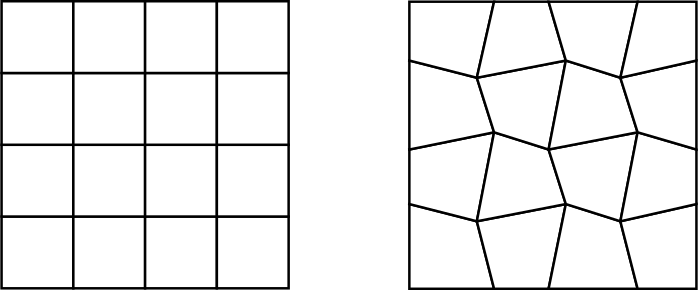
\includegraphics[width=4.0in]{figures/quadrilateral_patch_meshes.pdf}
    	\caption{Quadrilateral meshes: (left) regular, (right) distorted.}
    \label{fig:quadrilateral_patch_meshes}
\end{figure}

\begin{figure}[!h]
    \centering
    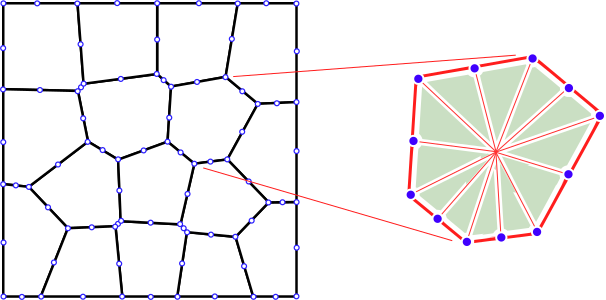
\includegraphics[width=4.0in]{figures/quadratic_polygonal_patch_mesh.pdf}
    	\caption{Patch of serendipity polygonal elements.}
    \label{fig:quadratic_polygonal_patch_mesh}
\end{figure}

Quadratic patch test errors for the FEM and DG-PEM were explored. The DG-PEM utilized an edge-based partitioning scheme and composite mid-point quadrature rules for each element. The DG-PEM bases was chosen such that $\varphi^h \in \mathcal{D}^h_2 (\Omega)$, yielding quadratically complete shape functions. Further, the DG-PEM was tested both with and without using the symmetric and nonsymmetric gradient correction schemes discussed previously. The results are presented in table \ref{tab:quadratic_patch_test}.

\begin{table}[!ht]
  \begin{center}
    \begin{tabular}{| c || c | c | c |}
    \hline
           & $E_2 (\Omega)$ & $||\mathbf{u}^h - \mathbf{u}|| / ||\mathbf{u}||$ & $||\boldsymbol{\sigma}^h - \boldsymbol{\sigma}|| / ||\boldsymbol{\sigma}||$ \\ \hline \hline
    FEM (regular 8-node quadrilaterals) & 9.0812E-016 & 1.7437E-009 & 1.3950E-008 \\ \hline
    FEM (distorted 8-node quadrilaterals) & 4.7831E-003 & 9.9714E-005 & 2.0795E-003 \\ \hline
    FEM (regular 9-node quadrilaterals) & 8.6713E-016 & 1.7437E-009 & 1.3950E-008 \\ \hline
    FEM (distorted 9-node quadrilaterals) & 1.2818E-015 & 2.0841E-009 & 1.5752E-008 \\ \hline
    DG-PEM (no gradient correction) & 3.3857E-008 & 9.8535E-002 & 2.8876E-001 \\ \hline
    DG-PEM (symmetric correction) & 3.6486E-007 & 3.5935E-008 & 1.4642E-007 \\ \hline
    DG-PEM (nonsymmetric correction) & 3.3857E-008 & 4.5498E-009 & 5.5341E-009 \\
    \hline
    \end{tabular}
    \caption{Quadratic patch test results comparison for FEM and DG-PEM.}
    \vspace{-5pt}
    \label{tab:quadratic_patch_test}
    \vspace{-25pt}
  \end{center}
\end{table}

It is interesting to note that the 8-node isoparametric quadrilaterals fail the quadratic patch test if the mesh becomes distorted. Only affinely distorted quadrilaterals of this type will exhibit quadratic completeness. Arbitrarily distorted elements will suffer from excessive interpolation errors, as observed in Table \ref{tab:quadratic_patch_test}. This behavior is discussed in greater detail in \cite{Arnold:02} and \cite{Arnold:01}. In comparison, the 9-node quadrilateral elements preserve quadratic completeness, even when distorted as in Figure \ref{fig:quadrilateral_patch_meshes}. However, it should be remarked that if the elements' edges are curved, both the 8- and 9-node isoparametric elements will lose 2nd order completeness and fail quadratic patch tests.

To account for the effects of integration error, the DG-PEM requires the use of a gradient correction scheme. However, if a symmetric correction scheme is employed, it is observed that there is a loss of completeness in the representation of the solution gradients over the element, corresponding to an increase in the interpolation error. Only the nonsymmetric gradient correction method is able to achieve the desired level of accuracy in the quadratic patch test. It shall therefore be used exclusively throughout the remainder of our discussions.

%Another quadratic patch test which involves no body force considers an elastic cantilever beam in pure bending, as depicted in Figure \ref{fig:bending_patch_test}. For clarity, this problem shall be referred to as the ``bending patch test.'' The support conditions of the (weakly) fixed beam are
%\begin{equation}
%	u_1 (X_1 = 0) = 0, \quad u_2 (X_1 = 0, X_2 = 0) = 0.
%\end{equation}
%A linearly varying traction $\bar{\mathbf{t}} = (M X_2, \, 0)$ is applied to the free end of the beam. For plane strain isotropic elasticity, the exact solution is:
%\begin{equation}
%	u_1 (\mathbf{X}) = \frac{M (\lambda + 2 \mu)}{4 \mu (\lambda + \mu)} X_1 X_2,
%\end{equation}
%\begin{equation}
%	u_2 (\mathbf{X}) = - \frac{M}{8 \mu (\lambda + \mu)} \left[ (\lambda + 2 \mu) X_1^2 + \lambda X_2^2 \right],
%\end{equation}
%\begin{equation}
%	\sigma_{11} = M X_2, \quad \sigma_{22} = \sigma_{12} = 0.
%\end{equation}

\section{Tests for Element Quality}

\subsection*{Conditioning of Individual Element Stiffness Matrices}

Partitioned element methods allow for the elements to take on virtually arbitrary shape. Nonetheless, elements with non-convex or degenerate features may degrade the overall accuracy of the resulting numerical solution. This section attempts to characterize the behavior of a representative sampling of polygonal PEM elements by examining the eigenvalues of each element's elastic stiffness matrix.

The motivation for the present study is to assess the effects of element formulation upon a given element's susceptibility to geometric locking phenomena. Heuristically: an element will be more sensitive to the effects of locking if its local stiffness matrix contains a number of eigenmodes (modes of deformation) whose corresponding eigenvalues are excessively large in comparison with the low-order deformation modes.

As a separate issue from locking, if a given element's local stiffness matrix is poorly conditioned, the global stiffness matrix of a mesh which contains said element may become poorly conditioned, as well. This may negatively impact the degree of solution accuracy that can be obtained due to floating point arithmetic. For implicit solid mechanics applications, the accuracy of any linear solver (whether direct or iterative) will be compromised by poor conditioning of the global stiffness matrix.

For the elements considered, a comparison study was carried out to examine differences in the eigenvalue spectra of elements whose stiffness matrices were computed using various element formulations. Specifically, approximations to harmonic shape functions were obtained for each element using the VETFEM, the CG-PEM, and the DG-PEM. These results were compared against a computed reference solution for the harmonic shape functions.

For each element, the elastic constants for Young's modulus and Poisson's ratio were chosen as $E = 1.0$ and $\nu = 0.0$, respectively. The choice of $\nu = 0.0$ is deliberate, and aims to decouple the effects of volumetric locking from the effects of geometric locking. All elements were scaled to have roughly unit diameter.

\subsubsection*{Examination of the Effects of Geometric Non-convexity}

A study was carried out to assess the effects of geometric non-convexity on a given element's eigenvalue spectrum. Three element shapes were considered, including: (A) a regular convex polygon, (B) an element with two collinear edges, and (C) a non-convex polygon. These elements are illustrated in Figure \ref{fig:concave_element_shapes}.

\begin{figure}[!h]
  \centering
  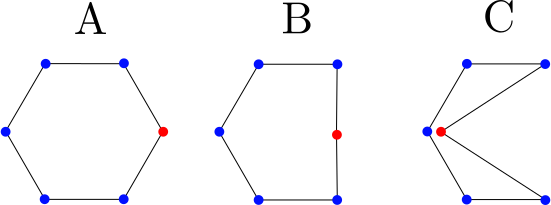
\includegraphics[width=3.5in]{figures/concave_element_shapes.pdf}  \caption{A representative sampling of hexagonal elements: (A) strictly convex, (B) two collinear edges, (C) non-convex.}
  \label{fig:concave_element_shapes}
\end{figure}

The harmonic shape functions defined on these elements were approximated using the VETFEM, the CG-PEM, and the DG-PEM. The VETFEM approximations consisted of 4th order polynomials, and were obtained as the solutions to (\ref{eq:vetfem}). The CG-PEM and DG-PEM approximations were obtained using the random Delaunay partitions shown in Figure \ref{fig:concave_element_partitions}. The penalty parameters appearing in (\ref{eq:penalty_parameters}) for the DG-PEM were chosen such that $\alpha_{0\gamma} = 10$, $\alpha_{1\gamma} = 0$ for all segments $\gamma$. Unless otherwise noted, the NIPG version of the DG-PEM (with $\epsilon = +1$) was utilized throughout. Reference solutions for the harmonic shape functions were computed on a highly refined partition of the element using the CG-PEM.

\begin{figure}[!h]
  \centering
  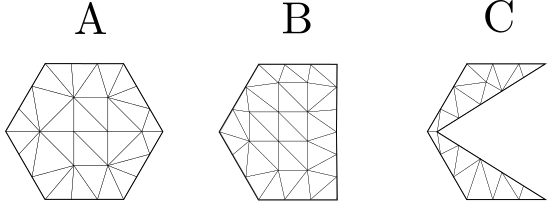
\includegraphics[width=3.5in]{figures/concave_element_partitions.pdf}  \caption{Delaunay partitions for elements A, B, and C.}
  \label{fig:concave_element_partitions}
\end{figure}

For the red nodes indicated in Figure \ref{fig:concave_element_shapes}, color plots of the associated harmonic shape functions (and their corresponding approximations) are provided in Figure \ref{fig:concave_element_comparison}.

\begin{figure}[!h]
  \centering
  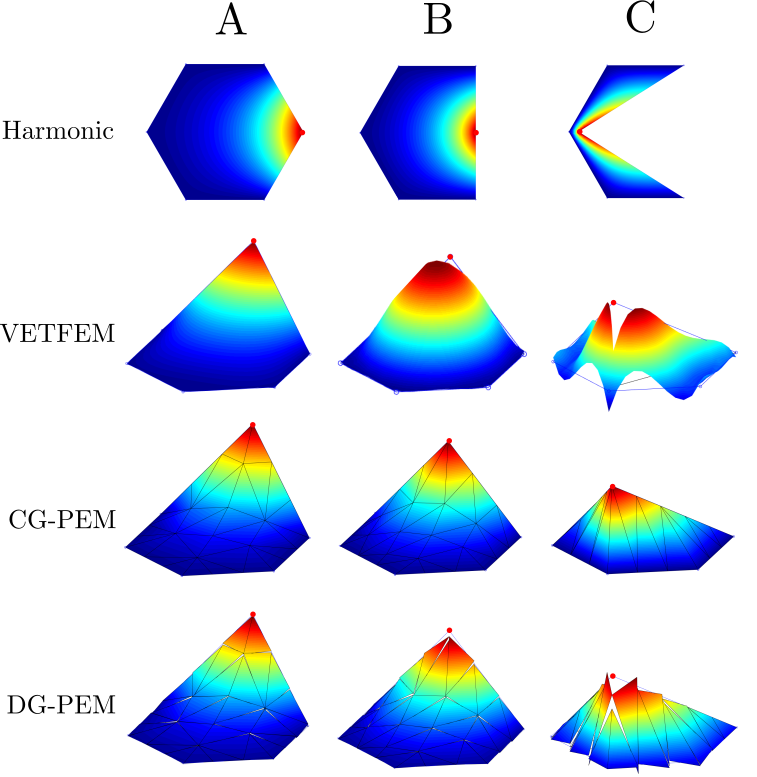
\includegraphics[width=5.0in]{figures/concave_element_comparison.pdf}  \caption{Comparison of the shape functions computed for elements A, B, and C using the VETFEM, CG-PEM, and DG-PEM.}
  \label{fig:concave_element_comparison}
\end{figure}

Concerning the VETFEM approximations depicted in Figure \ref{fig:concave_element_comparison} (particularly for elements B and C), the resulting shape functions present a number of undesirable features: oscillations, non-positivity, and non-interpolatory behavior. By comparison, the DG-PEM approximations avoid the issue of oscillations, though they are not strictly positive, nor are they interpolatory. Only the CG-PEM approximations can claim good behavior on all three fronts: they are non-oscillatory, strictly positive, and interpolatory. Nonetheless, it is important to emphasize that the aforementioned properties are not strictly necessary for convergence of the overall method. So long as a stable and consistent integration of the weak form is obtained, convergence is achieved. For certain applications, maintaining strict positivity or continuity of the shape function approximations may be desirable, though such applications are not considered here.

Using the aforementioned approximations in place of the harmonic shape functions, the elements' elastic stiffness matrices were computed (by numerical quadrature). The eigendecomposition of each element's local stiffness matrix was then determined, with particular attention paid to the largest eigenvalue $\lambda_{\max}$ and the smallest (non-zero) eigenvalue $\lambda_{\min}$. A comparison of the computed values for $\lambda_{\max}$ and $\lambda_{\min}$ is provided in table \ref{tab:concave_stiffness_max_min_eigenvalue}.

\begin{table}
\centering
\begin{subtable}{.5\textwidth}
\centering
\begin{tabular}{| c || c | c | c |}
    \hline
		Element  & A      & B      & C \\ \hline \hline
		Harmonic	 & 0.9635 & 1.2151 & 7.1166 \\ \hline
		VETFEM	 & 0.9950 & 4.4864 & 6.0305 \\ \hline
		CG-PEM	 & 1.0723 & 1.2760 & 8.7108 \\ \hline
		DG-PEM	 & 0.9668 & 1.1997 & 6.2766 \\
    \hline
    \end{tabular}
    \caption{Largest eigenvalue: $\lambda_{\max}$}
    \label{tab:concave_stiffness_max_eigenvalue}
\end{subtable}% <---- don't forget this %
\begin{subtable}{.5\textwidth}
\centering
\begin{tabular}{| c || c | c | c |}
    \hline
		Element  & A      & B      & C \\ \hline \hline
		Harmonic	 & 0.5226 & 0.3449 & 0.00562 \\ \hline
		VETFEM   & 0.5335 & 0.3491 & 0.09189 \\ \hline
		CG-PEM   & 0.6175 & 0.3935 & 0.00694 \\ \hline
		DG-PEM   & 0.5345 & 0.3425 & 0.00527 \\
    \hline
    \end{tabular}
    \caption{Smallest (non-zero) eigenvalue: $\lambda_{\min}$}
    \label{tab:concave_stiffness_min_eigenvalue}
\end{subtable}

\caption{Comparison of maximum and minimum (non-zero) eigenvalues of the element stiffness matrices for the elements shown in Figure \ref{fig:concave_element_shapes}.}
\label{tab:concave_stiffness_max_min_eigenvalue}
\end{table}

Irrespective of the chosen approximation method, the condition number for a given element's stiffness matrix becomes large as the degree of geometric non-convexity increases. The VETFEM yields a fairly accurate approximation for the eigenvalues of element A, but obtains an overly stiff approximation for element B, and overestimates the eigenvalues at the low end of the spectrum for element C. The CG-PEM appears to uniformly over-estimate the eigenvalue spectra of all elements A, B, and C, though not significantly. By contrast, the DG-PEM under-estimates the eigenvalues for elements B and C, though this behavior is observed to be contingent upon upon how the penalty parameters $\alpha_{0\gamma}$ and $\alpha_{1\gamma}$ are specified. Table \ref{tab:concave_stiffness_max_min_eigenvalue_parameter_study} illuminates the dependence of $\lambda_{\max}$ and $\lambda_{\min}$ (for element C) upon the choice of DG-PEM penalty parameters. Similar parameter dependencies are obtained for elements A and B.

\begin{table}
\centering
\begin{subtable}{1.0\textwidth}
\centering
\begin{tabular}{| c || c | c | c | c |}
    \hline
DG-PEM & $\alpha_{0\gamma} = 10^{-3}$ & $\alpha_{0\gamma} = 10^{0}$ & $\alpha_{0\gamma} = 10^{3}$ & $\alpha_{0\gamma} = 10^{6}$ \\ \hline \hline
$\alpha_{1\gamma} = 0.0$	& 5.9210 & 5.4949 & 8.6484 & 8.7108 \\ \hline
$\alpha_{1\gamma} = 10^{0}$ & 5.9210 & 5.2235 & 7.7525 & 8.7106 \\ \hline
$\alpha_{1\gamma} = 10^{3}$ & 5.9210 & 5.0938 & 3.9671 & 7.7874 \\ \hline
$\alpha_{1\gamma} = 10^{6}$ & 5.9210 & 5.0935 & 3.8699 & 3.9640 \\
    \hline
    \end{tabular}
    \caption{Largest eigenvalue: $\lambda_{\max}$}
    \label{tab:concave_stiffness_max_eigenvalue_parameter_study}
\end{subtable}% <---- don't forget this %
\\
\begin{subtable}{1.0\textwidth}
\centering
\begin{tabular}{| c || c | c | c | c |}
    \hline
DG-PEM & $\alpha_{0\gamma} = 10^{-3}$	&	$\alpha_{0\gamma} = 10^{0}$	&	$\alpha_{0\gamma} = 10^{3}$	&	$\alpha_{0\gamma} = 10^{6}$ \\ \hline \hline
$\alpha_{1\gamma} = 0.0$	&	0.004747	&	0.003554	&	0.006920	&	0.006943 \\ \hline
$\alpha_{1\gamma} = 10^{0}$	&	0.004748	&	0.003675	&	0.006489	&	0.006941 \\ \hline
$\alpha_{1\gamma} = 10^{3}$	&	0.004748	&	0.004210	&	0.002898	&	0.006508 \\ \hline
$\alpha_{1\gamma} = 10^{6}$	&	0.004748	&	0.004211	&	0.003660	&	0.002896 \\
    \hline
    \end{tabular}
    \caption{Smallest (non-zero) eigenvalue: $\lambda_{\min}$}
    \label{tab:concave_stiffness_min_eigenvalue_parameter_study}
\end{subtable}

\caption{Comparison of maximum and minimum (non-zero) eigenvalues of the element stiffness matrix for element C, computed for various DG-PEM penalty parameter values.}
\label{tab:concave_stiffness_max_min_eigenvalue_parameter_study}
\end{table}

The results in table \ref{tab:concave_stiffness_max_min_eigenvalue_parameter_study} warrant a number of observations. The eigenvalue spectrum obtained for the DG-PEM converges to that of the CG-PEM as the value of $\alpha_{0\gamma}$ is increased (provided $\alpha_{1\gamma}$ is sufficiently small). Moreover, the shape functions will themselves converge to the $C^0$ continuous approximations obtained by the CG-PEM. This is the expected result.
Additionally, if $\alpha_{0\gamma}$ is made sufficiently small, the eigenvalues will becomes relatively insensitive to the choice of $\alpha_{1\gamma}$. 

Conversely, as $\alpha_{0\gamma}$ is increased, the eigenvalues (and the corresponding shape function approximations) become more sensitive to the choice of $\alpha_{1\gamma}$. In such cases, $\alpha_{1\gamma}$ may be thought of as a ``regularization'' parameter, acting to effectively smooth out variations in the gradient of the shape functions over the element. For low-order DG-PEM, increasing $\alpha_{1\gamma}$ tends the element towards a uniform gradient formulation. Doing so risks rank-deficiency of the element's resulting stiffness matrix. If $\alpha_{0\gamma}$ and $\alpha_{1\gamma}$ are increased proportionally to one another, one recovers the behavior of the pure penalty DG-PEM corresponding to (\ref{eq:pure_penalty}).

\subsubsection*{Examination of the Effects of Nearly Degenerate Features}

A study was carried out to assess the effects of geometric degeneracy on a given element's eigenvalue spectrum. The two elements illustrated in Figure \ref{fig:degenerate_element_shapes} were considered: a regular pentagon, and an irregular pentagon with a comparatively short edge.

\begin{figure}[!h]
  \centering
  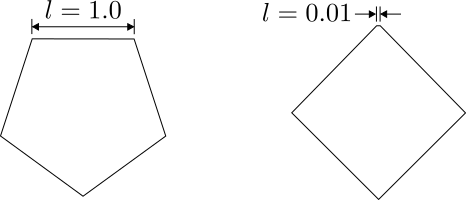
\includegraphics[width=3.7in]{figures/degenerate_element_shapes.pdf}  \caption{Two convex pentagonal elements: (left) regular pentagon with edges of length $l = 1.0$, (right) pentagon with a comparatively short edge of length $l = 0.01$.}
  \label{fig:degenerate_element_shapes}
\end{figure}

As in the previous example, the harmonic shape functions defined on these elements were approximated by the VETFEM (using 3rd order polynomials), the CG-PEM (using an edge-based partition), and the DG-PEM (using an edge-based partition, and the parameter settings described for the previous problem). Reference solutions for the harmonic shape functions were computed on a highly refined partition of the element using the CG-PEM.

\begin{figure}[!h]
  \centering
  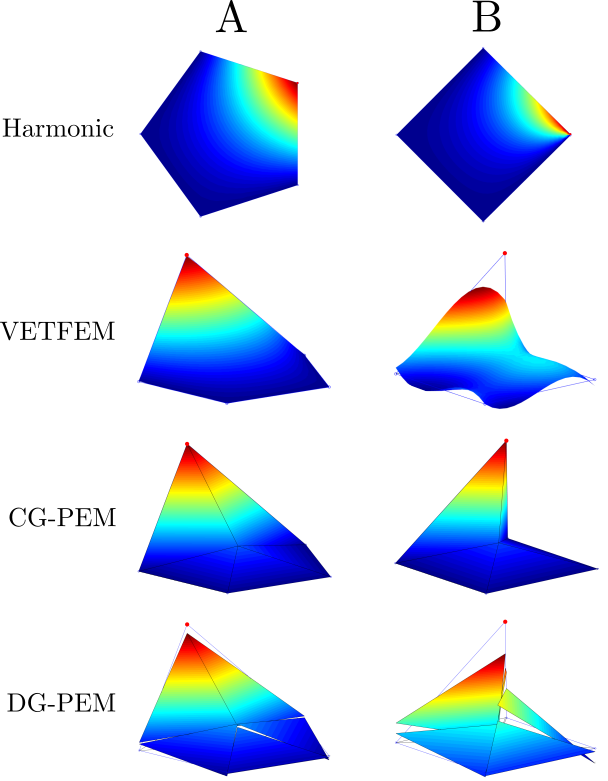
\includegraphics[width=5.0in]{figures/degenerate_element_comparison.pdf}  \caption{Comparison of shape functions computed for the two pentagonal elements with $l=1.0$ and $l=0.01$ using VETFEM, CG-PEM, and DG-PEM.}
  \label{fig:degenerate_element_comparison}
\end{figure}

As in the previous example, the aforementioned approximations were used in place of the harmonic shape functions when integrating the elements' elastic stiffness matrices. A comparison of the computed values for $\lambda_{\max}$ and $\lambda_{\min}$ is provided in table \ref{tab:degenerate_stiffness_max_min_eigenvalue}.

\begin{table}
\centering
\begin{subtable}{.5\textwidth}
\centering
\begin{tabular}{| c || c | c |}
    \hline
             & $l=1.0$ & $l=0.01$ \\ \hline \hline
    Harmonic & 0.9510 & 5.0899 \\ \hline
    VETFEM   & 0.9510 & 1.6818 \\ \hline
    CG-PEM   & 1.1326 & 64.098 \\ \hline
    DG-PEM   & 0.9510 & 1.3085 \\
    \hline
    \end{tabular}
    \caption{Largest eigenvalue: $\lambda_{\max}$}
    \label{tab:degenerate_stiffness_max_eigenvalue}
\end{subtable}% <---- don't forget this %
\begin{subtable}{.5\textwidth}
\centering
\begin{tabular}{| c || c | c |}
    \hline
             & $l=1.0$ & $l=0.01$ \\ \hline \hline
    Harmonic & 0.4925 & 0.3951 \\ \hline
    VETFEM   & 0.4906 & 0.3746 \\ \hline
    CG-PEM   & 0.8387 & 0.5516 \\ \hline
    DG-PEM   & 0.4739 & 0.2592 \\
    \hline
    \end{tabular}
    \caption{Smallest (non-zero) eigenvalue: $\lambda_{\min}$}
    \label{tab:degenerate_stiffness_min_eigenvalue}
\end{subtable}

\caption{Comparison of maximum and minimum (non-zero) eigenvalues of the element stiffness matrices computed for the elements shown in Figure \ref{fig:degenerate_element_shapes}.}
\label{tab:degenerate_stiffness_max_min_eigenvalue}
\end{table}

As noted in the previous example, the CG-PEM consistently over-estimates the eigenvalue spectra of the elements. Using a coarse (edge-based) partition further degrades the accuracy of the CG-PEM shape functions, to the extent that higher-order modes of deformation are severely over-stiff. Upon decreasing the edge length $l$ further, the maximum eigenvalue was observed to increase as $\lambda_{\max} \approx O (l^{-1})$. By comparison, the eigenvalue spectra for the VETFEM and DG-PEM remain small (well-conditioned), and relatively constant as $l \rightarrow 0$. The VETFEM, however, is observed to yield oscillatory solutions for the shape functions with decreasing $l$.

While the aforementioned insensitivity of the DG-PEM's eigenvalue spectra to short edges appears to be a desirable quality, it remains to be seen whether this is indeed the case. Correspondingly, the following series of investigations seeks to evaluate the implications of this property in a practical context.

\subsection*{Meshes Consisting of Elements with Degenerate Edges}

Consider the two square patches depicted in Figure \ref{fig:polygonal_patches}, each containing 1,000 polygonal elements. Both meshes were generated using PolyMesher, a polygonal meshing tool detailed in \cite{Talischi:12}. The Voronoi mesh in Figure \ref{fig:patch_mesh} was obtained by random point sampling process, and contains numerous elements with very short edges. The mesh in Figure \ref{fig:lloyd_mesh} was obtained after 100 iterations of Lloyd's algorithm (described in \cite{Talischi:12}). Any remaining short edges in the mesh were collapsed out. As noted in the figure, the resulting elements may possess extremely short edges, which can potentially degrade the quality of any finite element solution computed on the polygonal mesh. Herein, we will investigate the effects of having short edges within a given mesh.
\begin{figure}[!h]
    \centering
    \begin{subfigure}[b]{0.49\linewidth}
            \centering
            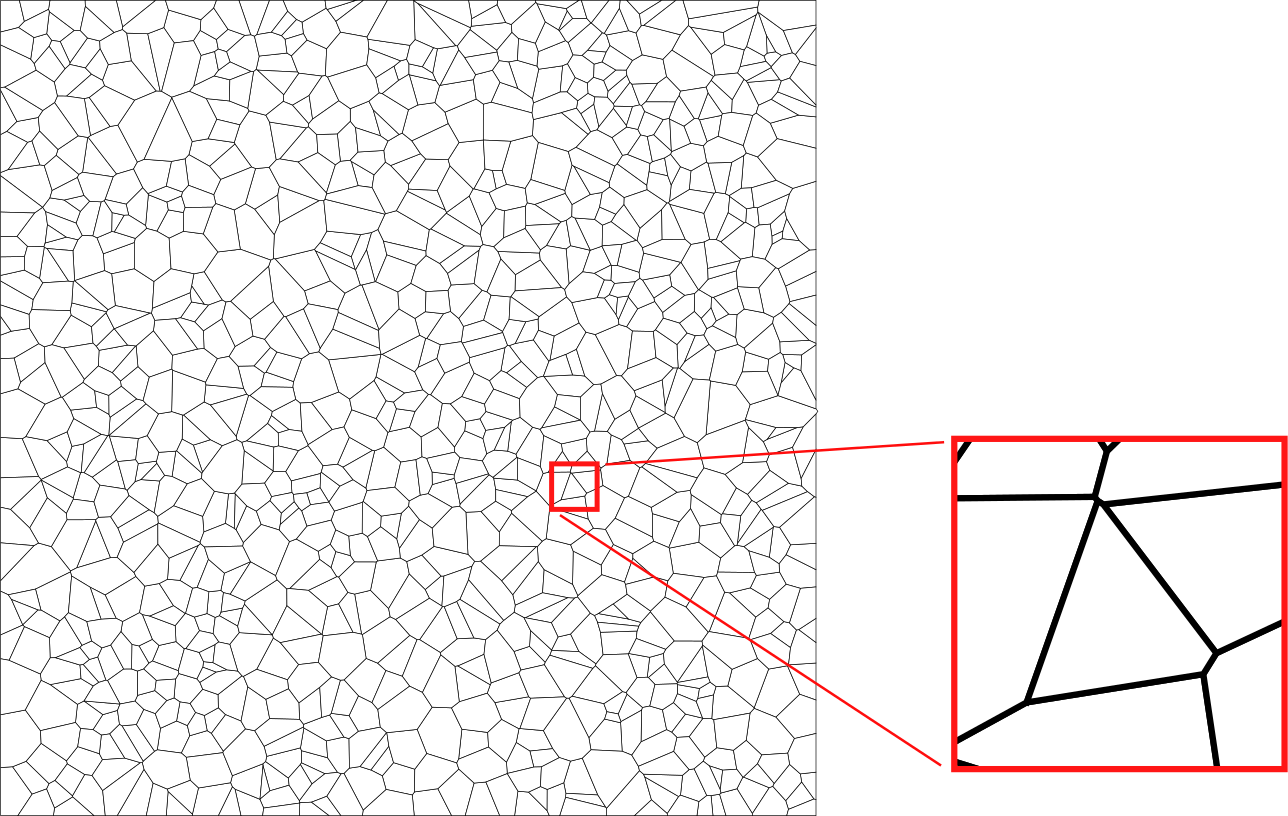
\includegraphics[width=3.0in]{figures/patch_mesh.pdf}
    			\caption{Random Voronoi mesh \label{fig:patch_mesh}}
    \end{subfigure}
	\begin{subfigure}[b]{0.49\linewidth}
            \centering
            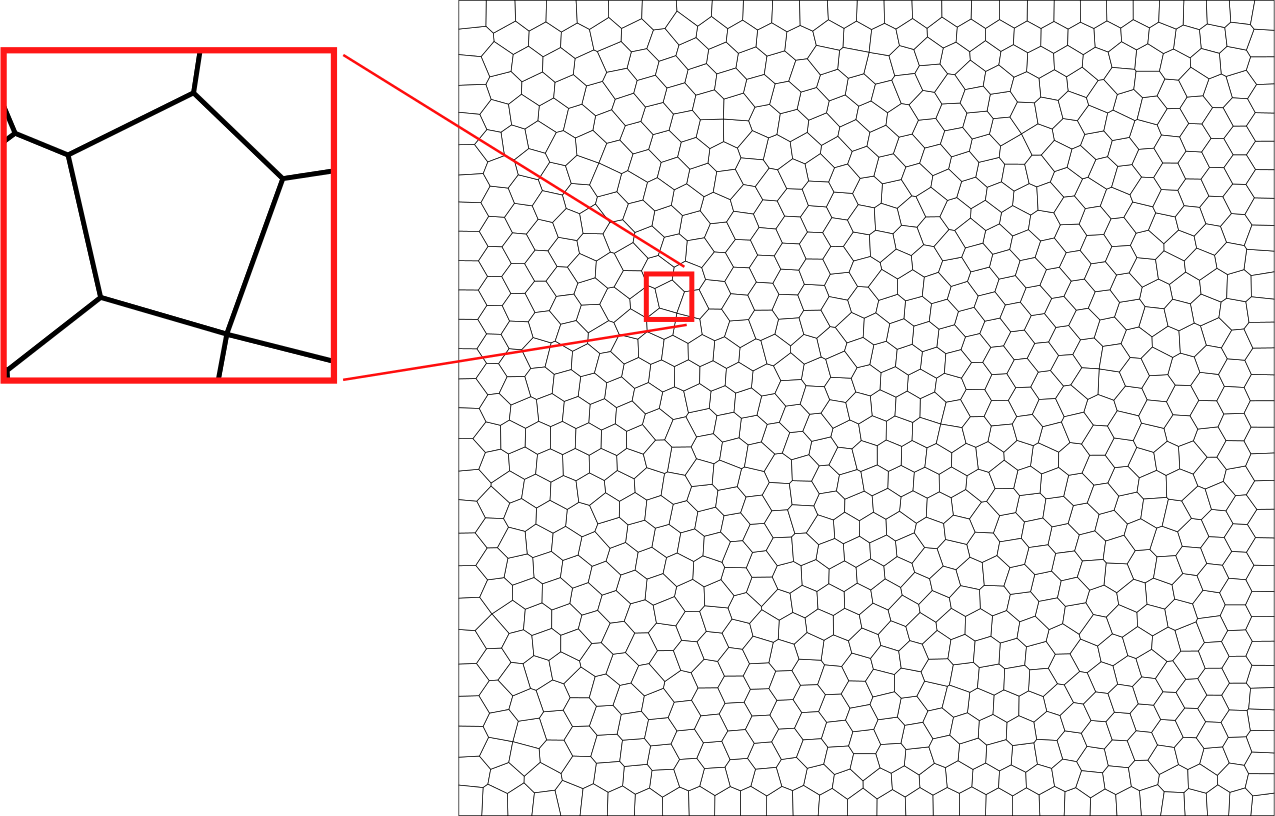
\includegraphics[width=3.0in]{figures/lloyd_mesh.pdf}
    			\caption{Lloyd mesh (100 iterations) \label{fig:lloyd_mesh}}
    \end{subfigure}
    \caption{Patches generated by PolyMesher, each containing 1,000 polygonal elements.}
    \label{fig:polygonal_patches}
\end{figure}

Some preliminary definitions are provided. For every polygonal element $\Omega_e \subset \mathbb{R}^2$, let $h_e$ denote the diameter of $\Omega_e$, such that
\begin{equation}
	h_e = \sup_{\mathbf{X}_1, \mathbf{X}_2 \in \Omega_e} || \mathbf{X}_1 - \mathbf{X}_2 ||_2.
\end{equation}
Further, denote by $|E|$ the length of any edge $E \subset \partial \Omega_e$, and define $\rho_e$ as the ratio of the smallest edge length $|E|$ divided by the element diameter $h_e$, i.e.
\begin{equation}
	\rho_e = \max_{E \subset \partial \Omega_e} \frac{|E|}{h_e}.
\end{equation}

For the mesh depicted in \ref{fig:polygonal_patches}, 
\begin{figure}[!h]
    \centering
    \begin{subfigure}[b]{0.49\linewidth}
            \centering
            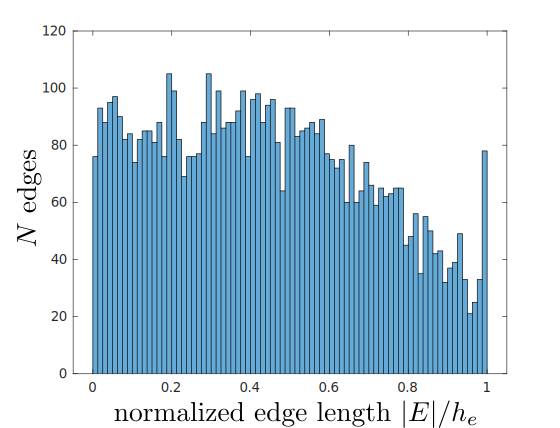
\includegraphics[width=3.0in]{figures/patch_edge_lengths.pdf}
    			\caption{Voronoi mesh \label{fig:patch_edge_lengths}}
    \end{subfigure}
	\begin{subfigure}[b]{0.49\linewidth}
            \centering
            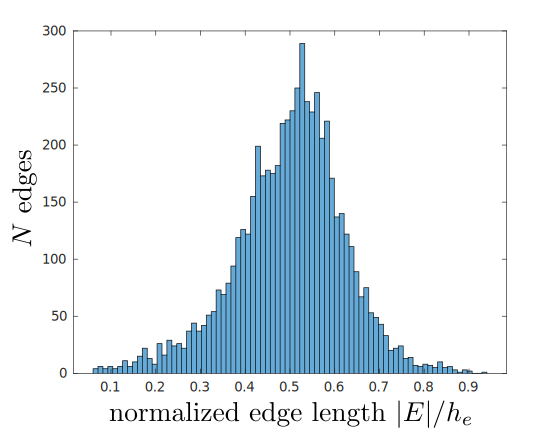
\includegraphics[width=3.0in]{figures/lloyd_edge_lengths.pdf}
    			\caption{Lloyd mesh \label{fig:lloyd_edge_lengths}}
    \end{subfigure}
    \begin{subfigure}[b]{0.49\linewidth}
            \centering
            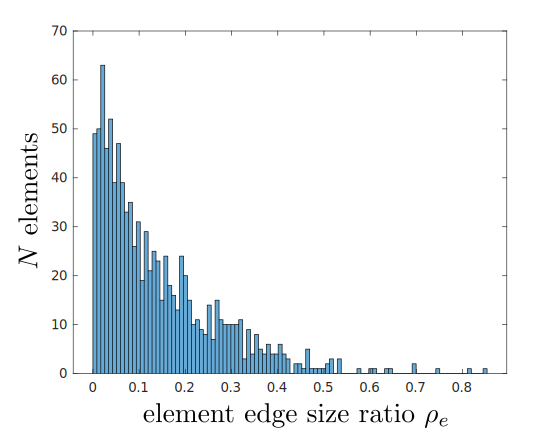
\includegraphics[width=3.0in]{figures/patch_edge_ratios.pdf}
    			\caption{Voronoi mesh \label{fig:patch_edge_ratios}}
    \end{subfigure}
	\begin{subfigure}[b]{0.49\linewidth}
            \centering
            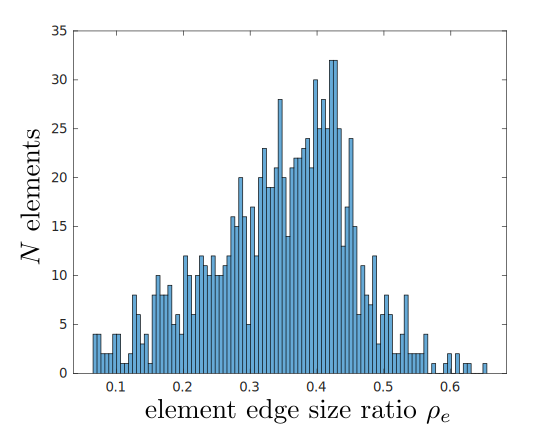
\includegraphics[width=3.0in]{figures/lloyd_edge_ratios.pdf}
    			\caption{Lloyd mesh \label{fig:lloyd_edge_ratios}}
    \end{subfigure}
    \caption{Histograms of various mesh metrics associated with the polygonal meshes depicted in Figure \ref{fig:polygonal_patches}:  (\subref{fig:patch_edge_lengths}) and (\subref{fig:lloyd_edge_lengths}) show the distributions of edge lengths contained in the random Voronoi and Lloyd meshes, respectively. (\subref{fig:patch_edge_ratios}) and (\subref{fig:lloyd_edge_ratios}) show the distributions for the smallest edge length ratios $\rho_e$ in the random Voronoi and Lloyd meshes, respectively.}
\end{figure}

\begin{figure}[!h]
  \centering
  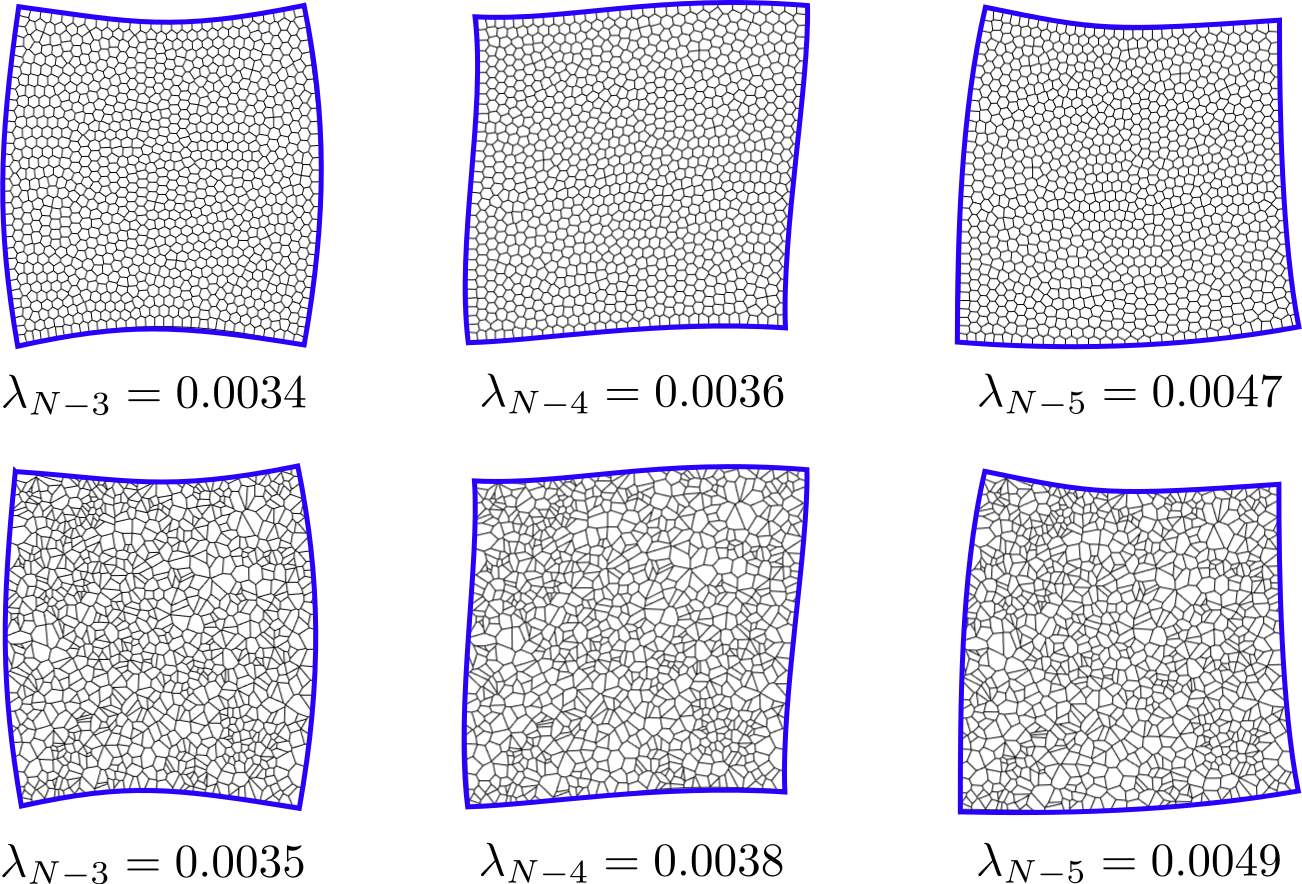
\includegraphics[width=5.0in]{figures/patch_eigenmodes_DGPEM.pdf}  \caption{Depiction of the smallest non-zero eigenvalues and corresponding eigenmodes.}
  \label{fig:patch_eigenmodes_DGPEM}
\end{figure}

\begin{table}[!ht]
  \begin{center}
    \begin{tabular}{| c || c | c |}
    \hline
           & Voronoi mesh & Lloyd mesh \\ \hline \hline
    FE-PEM & 9.1e+05 & 4.6e+03 \\ \hline
    DG-PEM ($\alpha_0 = 10^3$) & 4.8e+04 & 4.4e+03 \\ \hline
    DG-PEM ($\alpha_0 = 10^1$) & 1.0e+03 & 2.9e+03 \\ \hline
    DG-PEM ($\alpha_0 = 10^{-1}$) & 8.1e+02 & 2.7e+03 \\
    \hline
    \end{tabular}
    \caption{Computed values for the condition number $\kappa(\mathbf{K})$ of the global stiffness matrix $\mathbf{K}$ (excluding rigid body modes).}
    \vspace{-5pt}
    \label{tab:global_stiffness_condition_number}
    \vspace{-25pt}
  \end{center}
\end{table}

% FEPEM - lloyd
% Max E = 1.6e+1
% Mix E = 3.5e-03
% E Rat = 4.6e+03

% FEPEM - patch
% Max E = 3.0e+03
% Mix E = 3.3e-03
% E Rat = 9.1e+05
% Min Emodes:  0.0034, 0.0036, 0.0047

% DGPEM - lloyd - A0 = 1.0e+3
% Max E = 1.5e+1
% Mix E = 3.5e-03
% E Rat = 4.4e+03
% Min Emodes: 0.0035, 0.0038, 0.0049

% DGPEM - patch - A0 = 1.0e+3
% Max E = 1.6e+02
% Mix E = 3.3e-03
% E Rat = 4.8e+04

% DGPEM - lloyd - A0 = 1.0e+1
% Max E = 3.6e+00
% Mix E = 3.5e-03
% E Rat = 1.0e+03

% DGPEM - patch - A0 = 1.0e+1
% Max E = 9.6e+00
% Mix E = 3.3e-03
% E Rat = 2.9e+03

% DGPEM - lloyd - A0 = 1.0e-1
% Max E = 2.8e+00
% Mix E = 3.5e-03
% E Rat = 8.1e+02

% DGPEM - patch - A0 = 1.0e-1
% Max E = 8.9e+00
% Mix E = 3.3e-03
% E Rat = 2.7e+03

\begin{figure}[!h]
    \centering
    \begin{subfigure}[b]{0.49\linewidth}
            \centering
            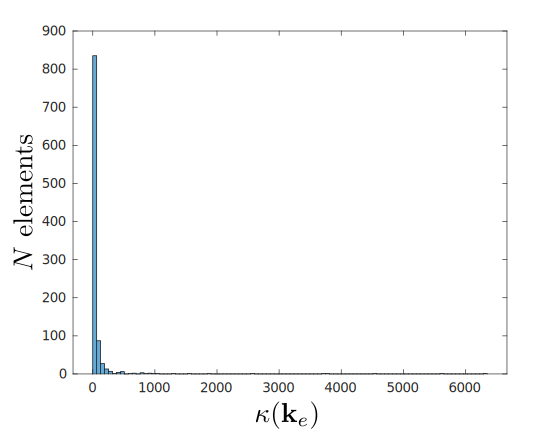
\includegraphics[width=3.0in]{figures/patch_condition_number_FEPEM.pdf}
    			\caption{CG-PEM on the Voronoi mesh  \label{fig:patch_condition_number_FEPEM}}
    \end{subfigure}
	\begin{subfigure}[b]{0.49\linewidth}
            \centering
            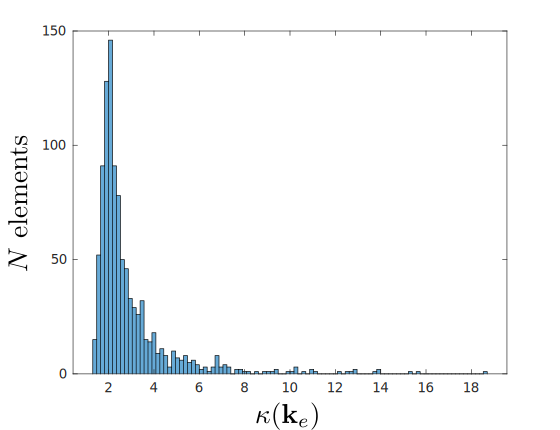
\includegraphics[width=3.0in]{figures/lloyd_condition_number_FEPEM.pdf}
    			\caption{CG-PEM on the Lloyd mesh  \label{fig:lloyd_condition_number_FEPEM}}
    \end{subfigure}
    \begin{subfigure}[b]{0.49\linewidth}
            \centering
            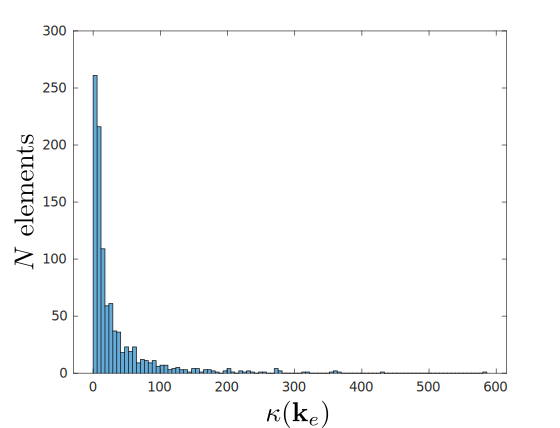
\includegraphics[width=3.0in]{figures/patch_condition_number_DGPEM.pdf}
    			\caption{DG-PEM on the Voronoi mesh  \label{fig:patch_condition_number_DGPEM}}
    \end{subfigure}
	\begin{subfigure}[b]{0.49\linewidth}
            \centering
            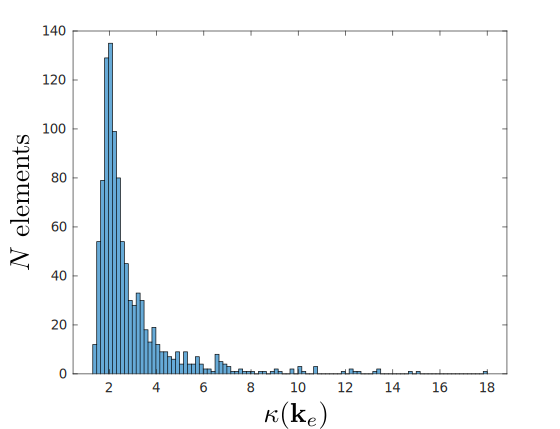
\includegraphics[width=3.0in]{figures/lloyd_condition_number_DGPEM.pdf}
    			\caption{DG-PEM on the LLoyd mesh  \label{fig:lloyd_condition_number_DGPEM}}
    \end{subfigure}
    \caption{Histograms of various element metrics associated with the polygonal meshes depicted in Figure \ref{fig:polygonal_patches}:  (\subref{fig:patch_edge_lengths}) and (\subref{fig:lloyd_edge_lengths}) show the distributions of edge lengths contained in the random Voronoi and Lloyd meshes, respectively; (\subref{fig:patch_edge_ratios}) and (\subref{fig:lloyd_edge_ratios}) show the distributions for the smallest edge length ratios $\rho_e$ in the random Voronoi and Lloyd meshes, respectively.}
\end{figure}

% local condition number investigation
	% look at DG-PEM system conditioning for certain degenerate elements
	%	* construct a random voronoi mesh on a 2d patch of elements
	%		- get edge-length metrics for voronoi cells
	%   		- examine condition number of local DGPEM systems on these elems
	%       - examine condition number of local stiffness matricies
	%			* look at max and min eigenvalues
	%		- check partition of unity and linear completeness passage
	%		- after grad correction, examine satisfaction of patch tests
	%	* do this for quadratic elements, as well
	%	* do parameter sensitivity analysis
	%	* look at global stiffness matrix condition number
	% look at conditioning for plate-like geometry (anisotropic patch tests)

% check via a series of single-element tests:
	% - examine a test involving a single non-convex element
	%   * shift node around, showing behavior vs. parameterized location
	%     - compare results for VETFEM, DGPEM, and FEPEM vs true harmonic SF
	%     - look at:
	%       * max and min eigenvalues of resulting stiffness matrix
	%       * comment on condition number, and effect on 
	%   * choose different partitioning algorithms / refinement levels
	%   * play around with DGPEM penalization parameters
	%   * examine effects of choosing DG
	% - do a test with a patch of non-convex elements
	%   * examine effects on global stiffness matrix conditioning
	%	* parameterized non-convexity, 

\section{Convergence Analysis}

\subsection*{Infinite Elastic Plate in Far-Field Tension}

\begin{figure}[!h]
  \centering
  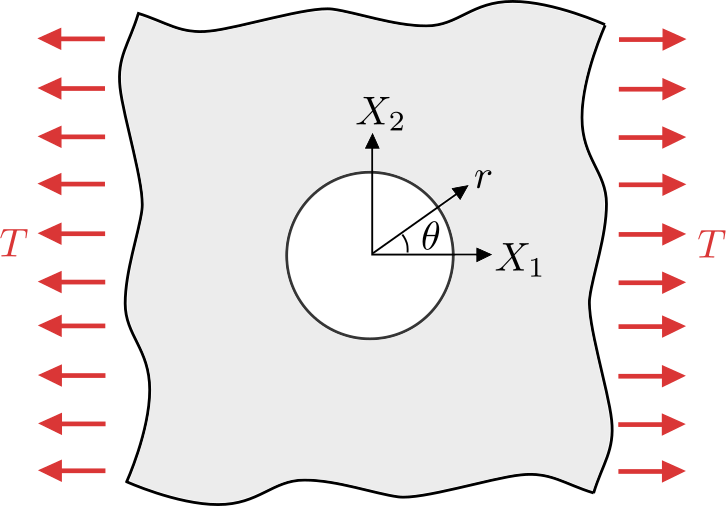
\includegraphics[width=4.0in]{figures/plate_with_hole.pdf}  \caption{Infinite plate with a circular hole placed in uniaxial tension.}
  \label{fig:plate_with_hole_problem}
\end{figure}
To demonstrate optimal convergence of the PEM for higher-order elements, we will choose to investigate the 2D elastostatics problem of an infinite plate with a circular hole in uniaxial tension (depicted in figure \ref{fig:plate_with_hole_problem}), for which there exist analytical solutions of the resulting displacement and stress fields (obtained from reference \cite{Wikiversity:17}):
\begin{equation}
  u_1 (r,\theta) = \frac{Ta}{8\mu} \left[ \frac{r}{a} (\kappa + 1) \cos \theta + \frac{2a}{r} ((1+\kappa) \cos \theta + \cos 3 \theta) - \frac{2a^3}{r^3} \cos 3 \theta \right]
\end{equation}
\begin{equation}
  u_2 (r,\theta) = \frac{Ta}{8\mu} \left[ \frac{r}{a} (\kappa - 3) \sin \theta + \frac{2a}{r} ((1-\kappa) \sin \theta + \sin 3 \theta) - \frac{2a^3}{r^3} \sin 3 \theta \right]
\end{equation}
\begin{equation}
  \sigma_{11} (r, \theta) = T - T \frac{a^2}{r^2} \bigg( \frac{3}{2} \cos 2 \theta + \cos 4 \theta \bigg) + T \frac{3a^4}{2r^4} \cos 4 \theta
\end{equation}
\begin{equation}
  \sigma_{22} (r, \theta) = - T \frac{a^2}{r^2} \bigg( \frac{1}{2} \cos 2 \theta - \cos 4 \theta \bigg) - T \frac{3a^4}{2r^4} \cos 4 \theta
\end{equation}
\begin{equation}
  \sigma_{12} (r, \theta) = - T \frac{a^2}{r^2} \bigg( \frac{1}{2} \sin 2 \theta + \sin 4 \theta \bigg) + T \frac{3a^4}{2r^4} \sin 4 \theta
\end{equation}
where $T$ is the far-field value of the applied tensile stress, $a$ is the radius of the circular hole centered at $r=0$, $\kappa = 4 - 3\nu$ (under plane-strain conditions), and $\nu$ and $\mu$ are the the Poisson's ratio and shear modulus of the material, respectively.

\begin{figure}[!h]
  \centering
  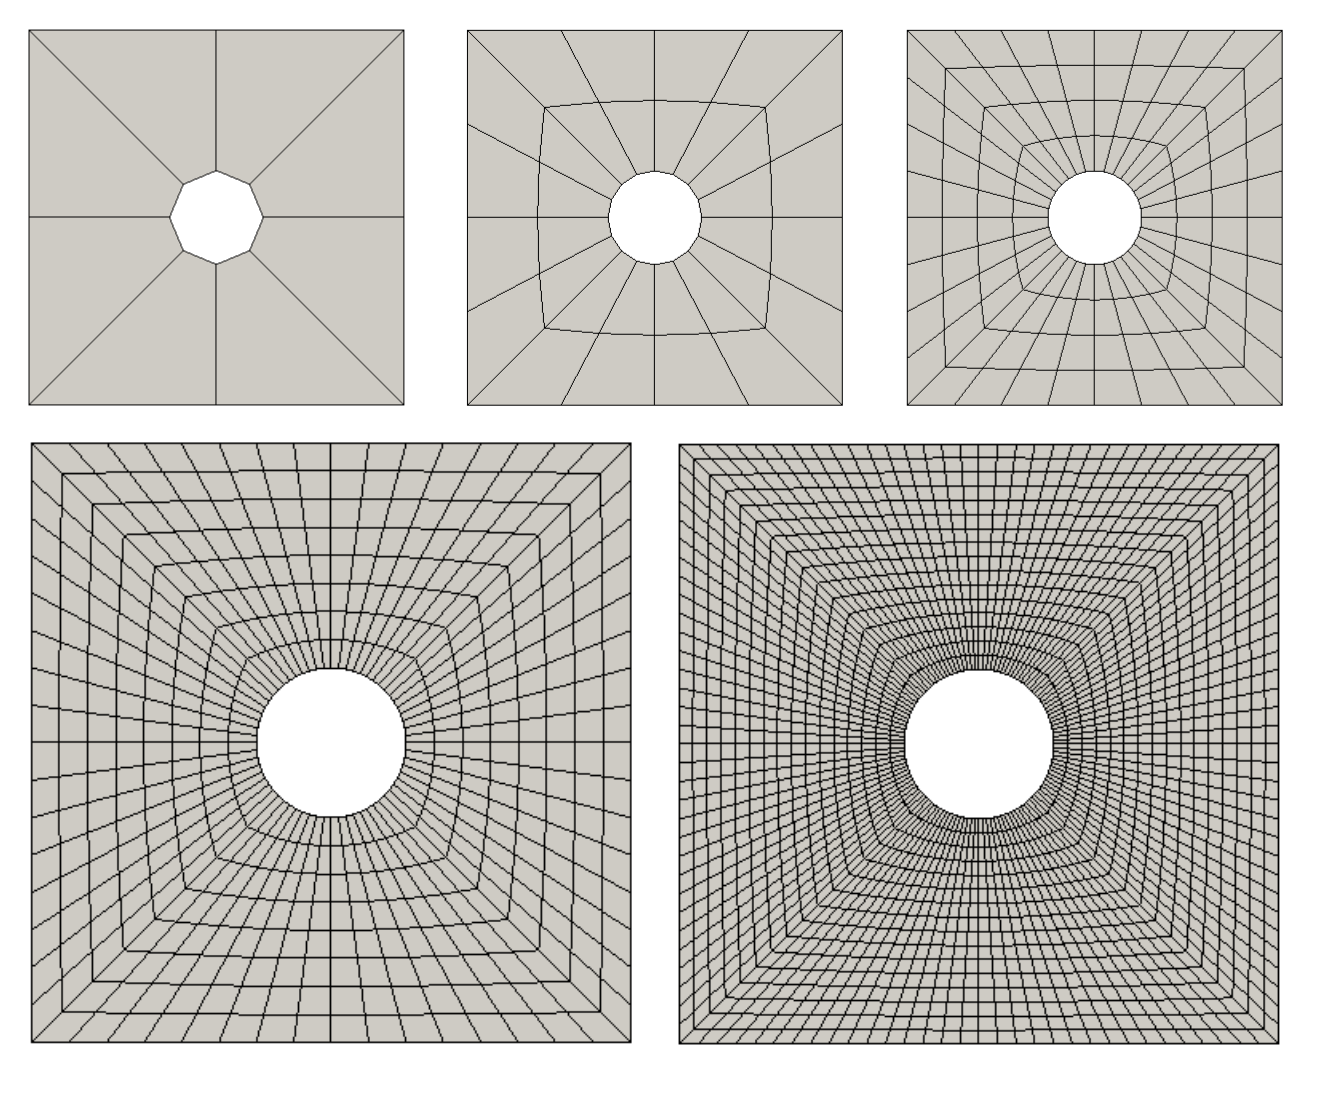
\includegraphics[width=6.0in]{figures/plate_with_hole_meshes.pdf}
  \caption{Quadrilateral meshes with varying levels of refinement.}
  \label{fig:plate_with_hole_meshes}
\end{figure}
A convergence study was carried out using a series of quadrilateral meshes with varying levels of refinement discretizing the restricted problem domain $X_i \in [ -1, +1]$ (see figure \ref{fig:plate_with_hole_meshes}.) The meshes consisted of either 4-node quadrilateral or 8-node serendipity quadrilateral elements, and employed either an isoparametric formulation, or a sufficiently high-order PEM formulation (i.e. $k=1$ for 4-node quadrilaterals, and $k=2$ for 8-node quadrilaterals.) Displacement boundary conditions were prescribed to be consistent with the exact solution on the restricted boundary. $L^2$ displacement error norms and $H^1$ energy error semi-norms were computed with reference to the exact solution, with the numerical results summarized in tables \ref{tab:l2_error}-\ref{tab:h1_rates}. The convergence rates in the $L^2$ and $H^1$ error norms are depicted in figures \ref{fig:l2_error} and \ref{fig:h1_error}, respectively.
\newpage
\begin{table}[!ht]
  \begin{center}
    \begin{tabular}{| c | c | c | c | c |}
    \hline
    $h$ & 4-node FEM & 4-node PEM & 8-node FEM & 8-node PEM \\ \hline
    1.2500 & 1.3133E-006 & 1.4901E-006 & 9.8369E-007 & 2.9990E-006 \\ \hline
    0.8006 & 6.9557E-007 & 9.8453E-007 & 4.8165E-007 & 1.3918E-006 \\ \hline
    0.4488 & 2.8755E-007 & 4.2859E-007 & 2.2034E-007 & 3.3673E-007 \\ \hline
    0.2371 & 1.0460E-007 & 1.3672E-007 & 8.1971E-008 & 4.8942E-008 \\ \hline
    0.1218 & 3.1430E-008 & 3.7296E-008 & 2.4628E-008 & 6.7201E-009 \\ \hline
    0.0617 & 8.3877E-009 & 9.5661E-009 & 6.5479E-009 & 1.6002E-009 \\
    \hline
    \end{tabular}
    \caption{Computed $L^2$ displacement error norms.}
    \vspace{-5pt}
    \label{tab:l2_error}
    \vspace{-25pt}
  \end{center}
\end{table}
\begin{table}[!ht]
  \begin{center}
    \begin{tabular}{| c | c | c | c | c |}
    \hline
    $h$ & 4-node FEM & 4-node PEM & 8-node FEM & 8-node PEM \\ \hline
    1.2500 &	-	&	-	&	-	&       -      \\ \hline
    0.8006 &	1.4265	&	0.9302	&	1.6028	&	1.7230 \\ \hline
    0.4488 &	1.5262	&	1.4369	&	1.3512	&	2.4518 \\ \hline
    0.2371 &	1.5848	&	1.7906	&	1.5496	&	3.0225 \\ \hline
    0.1218 &	1.8051	&	1.9502	&	1.8053	&	2.9808 \\ \hline
    0.0617 &	1.9424	&	2.0007	&	1.9479	&	2.1100 \\
    \hline
    \end{tabular}
    \caption{Computed $L^2$ displacement error norm convergence rates.}
    \vspace{-5pt}
    \label{tab:l2_rates}
    \vspace{-25pt}
  \end{center}
\end{table}
\begin{table}[!ht]
  \begin{center}
    \begin{tabular}{| c | c | c | c | c |}
    \hline
    $h$ & 4-node FEM & 4-node PEM & 8-node FEM & 8-node PEM \\ \hline
    1.2500 & 2.1468E-001 & 2.8913E-001 & 1.8275E-001 & 5.3700E-001 \\ \hline
    0.8006 & 1.8622E-001 & 2.5620E-001 & 1.5959E-001 & 3.0529E-001 \\ \hline
    0.4488 & 1.3786E-001 & 1.7930E-001 & 1.2495E-001 & 1.5310E-001 \\ \hline
    0.2371 & 9.2075E-002 & 1.1251E-001 & 7.9144E-002 & 5.8671E-002 \\ \hline
    0.1218 & 5.2124E-002 & 6.2223E-002 & 4.2868E-002 & 1.5541E-002 \\ \hline
    0.0617 & 2.7048E-002 & 3.2135E-002 & 2.1789E-002 & 3.3672E-003 \\
    \hline
    \end{tabular}
    \caption{Computed $H^1$ energy error semi-norms.}
    \vspace{-5pt}
    \label{tab:h1_error}
    \vspace{-25pt}
  \end{center}
\end{table}
\begin{table}[!ht]
  \begin{center}
    \begin{tabular}{| c | c | c | c | c |}
    \hline
    $h$ & 4-node FEM & 4-node PEM & 8-node FEM & 8-node PEM \\ \hline
    1.2500 &	-	&	-	&	-	&       -      \\ \hline
    0.8006 &	0.3192	&	0.2714	&	0.3042	&	1.2675 \\ \hline
    0.4488 &	0.5195	&	0.6166	&	0.4228	&	1.1924 \\ \hline
    0.2371 &	0.6326	&	0.7303	&	0.7156	&	1.5031 \\ \hline
    0.1218 &	0.8542	&	0.8892	&	0.9205	&	1.9944 \\ \hline
    0.0617 &	0.9646	&	0.9716	&	0.9950	&	2.2488 \\
    \hline
    \end{tabular}
    \caption{Computed $H^1$ energy error semi-norm convergence rates.}
    \vspace{-5pt}
    \label{tab:h1_rates}
    \vspace{-25pt}
  \end{center}
\end{table}

\begin{figure}[!h]
  \centering
    \begin{subfigure}[b]{0.49\linewidth}
            \centering
            \includegraphics[width=3.3in]{figures/plate_with_hole_quad_l2_error.pdf}
    			\caption{displacement error \label{fig:plate_with_hole_quad_l2_error}}
    \end{subfigure}
	\begin{subfigure}[b]{0.49\linewidth}
            \centering
            \includegraphics[width=3.3in]{figures/plate_with_hole_quad_h1_error.pdf}
    			\caption{stress error \label{fig:plate_with_hole_quad_h1_error}}
    \end{subfigure} \caption{Convergence plots for the plate with hole problem using standard isoparametric elements.}
  \label{fig:plate_with_hole_quad_error}
\end{figure}

\begin{figure}[!h]
  \centering
    \begin{subfigure}[b]{0.49\linewidth}
            \centering
            \includegraphics[width=3.3in]{figures/plate_with_hole_pem_l2_error.pdf}
    			\caption{displacement error \label{fig:plate_with_hole_pem_l2_error}}
    \end{subfigure}
	\begin{subfigure}[b]{0.49\linewidth}
            \centering
            \includegraphics[width=3.3in]{figures/plate_with_hole_pem_h1_error.pdf}
    			\caption{stress error \label{fig:plate_with_hole_pem_h1_error}}
    \end{subfigure} \caption{Convergence plots for the plate with hole problem using DG-PEM elements.}
  \label{fig:plate_with_hole_pem_error}
\end{figure}

A number of observations should be made regarding the resulting data. In particular, it is worthwhile to note that part of the incurred solution error may be attributable to the inexact representation of the problem geometry, especially for the coarse meshes. This may in part explain why the observed convergence rates are lower at coarser levels of refinement, but approach the expected rates as the mesh is further refined.

Additionally, we remark that isoparametric serendipity quadrilateral elements converge at sub-optimal rates if the elements are distorted in a non-affine fashion (as is the case for our meshes). This is an altogether expected result, and has been discussed in references \cite{Arnold:01} and \cite{Arnold:02}.

Conversely, we observe that the PEM quadrilateral elements converge at the optimal rates in both the $L^2$ and $H^1$ error norms, as we would hope.

Further work will seek to investigate the measured error and convergence rates of the PEM when the elements take on arbitrary shape, and for a variety of different formulations and penalization parameter settings.

\section{Parameter Sensitivity Analysis}

\section{Computational Efficiency}
\subsection{Performance Comparison}

\section{Resistance to Locking Phenomena}

\subsection*{Twisting Annulus}

Consider an incompressible elastic annulus whose inner radius at $r = R_i$ is fixed, and whose outer radius $r = R_o$ rigidly rotates at an angular velocity of $\Phi$. The radially symmetric displacement boundary conditions for this motion are described by
\begin{equation}
	u_r (R_i,t) = u_r (R_o,t) = 0, \quad u_z (R_i,t) = u_z (R_o,t) = 0,
\end{equation}
\begin{equation}
	u_\theta (R_i,t) = 0, \quad u_\theta (R_o,t) = R_o \, \Phi \, t,
\end{equation}
for all $t \geq 0$.

The elastic material is characterized by a linear hypoelastic material model of grade zero, obeying
\begin{equation}
  \dot{\boldsymbol{\sigma}} = \mathbb{C} : \mathbf{D} + \mathbf{W} \boldsymbol{\sigma} - \boldsymbol{\sigma} \mathbf{W},
\end{equation}

\subsubsection*{Exact Solution}

An exact solution for the aforementioned problem may be obtained by considering the stress divergence equations in cylindrical polar coordinates:
\begin{equation}
  \nabla \cdot \boldsymbol{\sigma} = \left\{ \begin{array}{c} \frac{\partial \sigma_{rr}}{\partial r} + \frac{\sigma_{rr}}{r} + \frac{1}{r} \frac{\partial \sigma_{\theta r}}{\partial \theta} + \frac{\partial \sigma_{z r}}{\partial z} - \frac{\sigma_{\theta \theta}}{r} \\
    \frac{1}{r} \frac{\partial \sigma_{\theta \theta}}{\partial \theta} + \frac{\partial \sigma_{r\theta}}{\partial r} + \frac{\sigma_{r\theta}}{r} + \frac{\sigma_{\theta r}}{r} + \frac{\partial \sigma_{z \theta}}{\partial z} \\
    \frac{\partial \sigma_{z z}}{\partial z} + \frac{\partial \sigma_{r z}}{\partial r} + \frac{\sigma_{r z}}{r} + \frac{1}{r} \frac{\partial \sigma_{\theta z}}{\partial \theta} \end{array} \right\} = \mathbf{0}.
\end{equation}
By the assumptions of plane strain and axisymmetry, we rationalize that $\boldsymbol{\sigma} (r)$ is a function of $r$, alone, and therefore,
\begin{equation}
  \nabla \cdot \boldsymbol{\sigma} = \left\{ \begin{array}{c} \frac{\partial \sigma_{rr}}{\partial r} + \frac{\sigma_{rr} - \sigma_{\theta \theta}}{r} \\
    \frac{\partial \sigma_{r\theta}}{\partial r} + \frac{2 \sigma_{r\theta}}{r} \\
    \frac{\partial \sigma_{r z}}{\partial r} + \frac{\sigma_{r z}}{r} \end{array} \right\} = \mathbf{0}.
\end{equation}
Furthermore, by the assumptions of plane strain, we observe that $\sigma_{rz} = 0$ and $\sigma_{\theta z} = 0$. Additionally, if we impose the incompressibility condition $\nabla \cdot \mathbf{v} = \text{tr} (\mathbf{D}) = 0$, we find that
\begin{equation}
  \text{tr} (\dot{\boldsymbol{\sigma}}) = 0 \, \Rightarrow \, \text{tr} (\boldsymbol{\sigma}) = 0 \, \forall t.
\end{equation}
The deformation necessitates that $\sigma_{zz} = 0$, and therefore $\sigma_{\theta \theta} = - \sigma_{rr}$. Consequently, we are left with 2 governing differential equations for $\sigma_{rr}$ and $\sigma_{r \theta}$:
\begin{equation}
  \frac{\partial \sigma_{rr}}{\partial r} + \frac{2 \sigma_{rr}}{r} = 0, \quad \frac{\partial \sigma_{r\theta}}{\partial r} + \frac{2 \sigma_{r\theta}}{r} = 0,
\end{equation}
whose solutions are of the form
\begin{equation}
  \sigma_{rr} = \frac{a}{r^2}, \quad \sigma_{r\theta} = \frac{b}{r^2}.
\end{equation}
Consequently,
\begin{equation}
  \left\{ \begin{array}{c} \sigma_{rr} \\ \sigma_{\theta \theta} \\ \sigma_{r \theta} \end{array} \right\} = r^{-2} \left\{ \begin{array}{c} +a \\ -a \\ b \end{array} \right\}.
\end{equation}

Under the assumption of incompressibility, we may characterize the deformation via the velocity field $v_r = 0$, $v_z = 0$, and $v_\theta (r) = r \dot{\phi}(r)$, yielding the velocity gradient (in cylindrical polar coordinates):
\begin{equation}
  \mathbf{L} = \nabla \mathbf{v} = \left[ \begin{array}{ccc} v_{r,r} & v_{r,\theta}/r-v_\theta /r & v_{r,z} \\
      v_{\theta,r} & v_{\theta,\theta}/r + v_r /r & v_{\theta,z} \\
      v_{z,r} & v_{z,\theta} /r & v_{z,z} \end{array} \right] = 
  \left[ \begin{array}{ccc} 0 & -\dot{\phi} & 0 \\
      \dot{\phi} + r \dot{\phi}_{,r} & 0 & 0 \\
      0 & 0 & 0 \end{array} \right],
\end{equation}
and the corresponding rate of deformation and spin tensors:
\begin{equation}
  \mathbf{D} = \frac{r \dot{\phi}_{,r}}{2} \left[ \begin{array}{ccc} 0 & 1 & 0 \\
      1 & 0 & 0 \\
      0 & 0 & 0 \end{array} \right], \quad \mathbf{W} = 
  \frac{2 \dot{\phi} + r \dot{\phi}_{,r}}{2} \left[ \begin{array}{ccc} 0 & - 1 & 0 \\
      1 & 0 & 0 \\
      0 & 0 & 0 \end{array} \right].
\end{equation}
The resulting stress rate equations are
\begin{equation}
  \left\{ \begin{array}{c} \dot{\sigma}_{rr} \\ \dot{\sigma}_{\theta \theta} \\ \dot{\sigma}_{r \theta} \end{array} \right\} = \left\{ \begin{array}{c} 0 \\ 0 \\ \mu r \dot{\phi}_{,r} \end{array} \right\} + 
  (2 \dot{\phi} + r \dot{\phi}_{,r}) \left\{ \begin{array}{c} - \sigma_{r \theta} \\ \sigma_{r \theta} \\ \sigma_{rr} \end{array} \right\},
\end{equation}
or
\begin{equation}
  \left\{ \begin{array}{c} \dot{a} \\ \dot{b} \end{array} \right\} = \left\{ \begin{array}{c} 0 \\ \mu r^3 \dot{\phi}_{,r} \end{array} \right\} + (2 \dot{\phi} + r \dot{\phi}_{,r}) \left[ \begin{array}{cc} 0 & -1 \\ 1 & 0 \end{array} \right] \left\{ \begin{array}{c} a \\ b \end{array} \right\},
\end{equation}
which must be valid $\forall r, \, t$. If we assume that $\dot{\phi} = f(r)$ is a function of $r$ (and not of $t$), then we obtain the condition
\begin{equation}
  3 f_{,r} + r f_{,rr} = 0,
\end{equation}
implying $f_{,r} = B r^{-3}$, and $\phi (r, t) = (A - B r^{-2} / 2)t$, thus
\begin{equation}
  \left\{ \begin{array}{c} \dot{a} \\ \dot{b} \end{array} \right\} = \left\{ \begin{array}{c} 0 \\ \mu B \end{array} \right\} + 2 A \left[ \begin{array}{cc} 0 & -1 \\ 1 & 0 \end{array} \right] \left\{ \begin{array}{c} a \\ b \end{array} \right\},
\end{equation}
and
\begin{equation}
  a(t) = - \frac{\mu B}{2 A} - C_2 \sin (2 A t) + C_1 \cos (2 A t),
\end{equation}
\begin{equation}
  b(t) = C_1 \sin (2 A t) + C_2 \cos (2 A t).
\end{equation}
Imposing the initial conditions $a(0) = b(0) = 0$ results in:
\begin{equation}
  a(t) = \frac{\mu B}{2 A} \left[ \cos (2 A t) - 1 \right], \quad b(t) = \frac{\mu B}{2 A} \sin (2 A t).
\end{equation}
Imposing the boundary conditions $\phi(R_i,t) = 0 \, \, \forall t$, $\phi(R_o,t) = \Phi \, t \, \, \forall t$ yields:
\begin{equation}
  A = \frac{\Phi R_i^{-2}}{R_i^{-2} - R_o^{-2}}, \quad B = \frac{2 \Phi}{R_i^{-2} - R_o^{-2}}.
\end{equation}

The final analytical solution for the displacement and stress fields is presented below:
\begin{equation}
  u_r = 0, \quad u_\theta = r \Phi \frac{R_i^{-2} - r^{-2}}{R_i^{-2} - R_o^{-2}} t, \quad u_z = 0,
\end{equation}
\begin{equation}
  \sigma_{rr} = - \sigma_{\theta \theta} = \mu \frac{r^{-2}}{R_i^{-2}} \left[ \cos \left( 2 \frac{\Phi R_i^{-2}}{R_i^{-2} - R_o^{-2}} t \right) - 1 \right],
\end{equation}
\begin{equation}
  \sigma_{r \theta} = \mu \frac{r^{-2}}{R_i^{-2}} \sin \left( 2 \frac{\Phi R_i^{-2}}{R_i^{-2} - R_o^{-2}} t \right).
\end{equation}

\subsubsection*{Numerical Results}

Because the element formulations that will be used herein possess only displacement degrees of freedom, we expect the finite element solutions to present inaccuracies due to the effects of volumetric locking. Moreover, it is not possible to run an analysis for a truly incompressible material (if the grade zero hypoelasticity model is to be utilized). For this reasons, it will suffice to examine solutions in the near-incompressible regime (i.e. $\nu = 0.4999$).

Additionally, because an accurate prediction of the pressure field requires the use of a mixed formulation, we expect the stress error to be dominated by errors in the pressure field. For this reason, we will choose to examine only the errors in the deviatoric stress field, where $s_{ij} = \sigma_{ij} - \frac{1}{3} \delta_{ij} \sigma_{kk}$ denotes the stress deviator.

\begin{figure}[!h]
  \centering
  \includegraphics[width=6.0in]{figures/annulus_meshes.pdf}
  \caption{Polygonal meshes with varying levels of refinement for the twisting annulus problem.}
  \label{fig:annulus_meshes}
\end{figure}

\begin{figure}[!h]
  \centering
  \includegraphics[width=6.0in]{figures/quad_annulus_meshes.pdf}
  \caption{Quadrilateral meshes with varying levels of refinement for the twisting annulus problem.}
  \label{fig:quad_annulus_meshes}
\end{figure}

\begin{figure}[!h]
  \centering
    \begin{subfigure}[b]{0.49\linewidth}
            \centering
            \includegraphics[width=3.3in]{figures/quad_l2_error.pdf}
    			\caption{displacement error \label{fig:quad_l2_error}}
    \end{subfigure}
	\begin{subfigure}[b]{0.49\linewidth}
            \centering
            \includegraphics[width=3.3in]{figures/quad_h1_error.pdf}
    			\caption{stress deviator error \label{fig:quad_h1_error}}
    \end{subfigure} \caption{Convergence plots for the twisting annulus problem using standard isoparametric elements.}
  \label{fig:quad_error}
\end{figure}

\begin{figure}[!h]
  \centering
    \begin{subfigure}[b]{0.49\linewidth}
            \centering
            \includegraphics[width=3.3in]{figures/quad_l2_error.pdf}
    			\caption{displacement error \label{fig:quad_l2_error}}
    \end{subfigure}
	\begin{subfigure}[b]{0.49\linewidth}
            \centering
            \includegraphics[width=3.3in]{figures/quad_h1_error.pdf}
    			\caption{stress deviator error \label{fig:quad_h1_error}}
    \end{subfigure} \caption{Convergence plots for the twisting annulus problem using standard isoparametric elements.}
  \label{fig:quad_error}
\end{figure}

\subsection*{Thin Corner-Supported Plate}

Consider a thin plate 
(Description of the corner-supported plate problem).

\begin{figure}[!h]
  \centering
  \includegraphics[width=6.0in]{figures/plate_meshes.pdf}
  \caption{Hexahedral meshes with variable plate thickness $h$ and mesh perturbations $p$ for the corner-supported plate problem.}
  \label{fig:plate_meshes}
\end{figure}

\subsubsection{Exact Solution}

An exact solution for the vertical displacement field of the plate prob

\section{Comparison with Isoparametric Finite Elements}

\subsection*{Ductile Necking}

\begin{figure}[!h]
    \centering
    \begin{subfigure}[b]{0.49\linewidth}
            \centering
            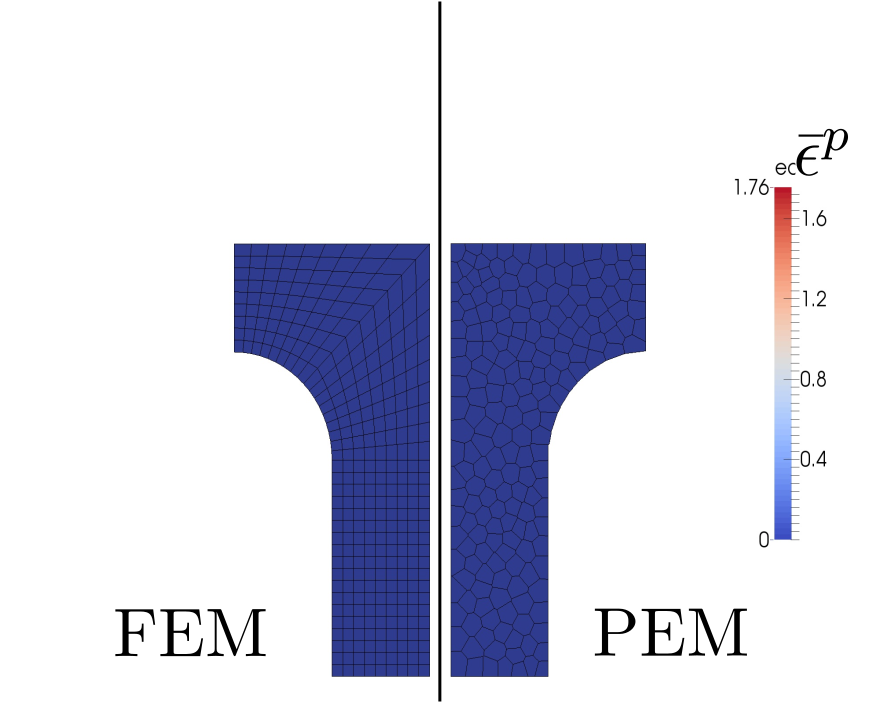
\includegraphics[width=3.0in]{figures/necking_eqps_0.pdf}
    			\caption{$t=0.0$ \label{fig:necking_eqps_0}}
    \end{subfigure}
	\begin{subfigure}[b]{0.49\linewidth}
            \centering
            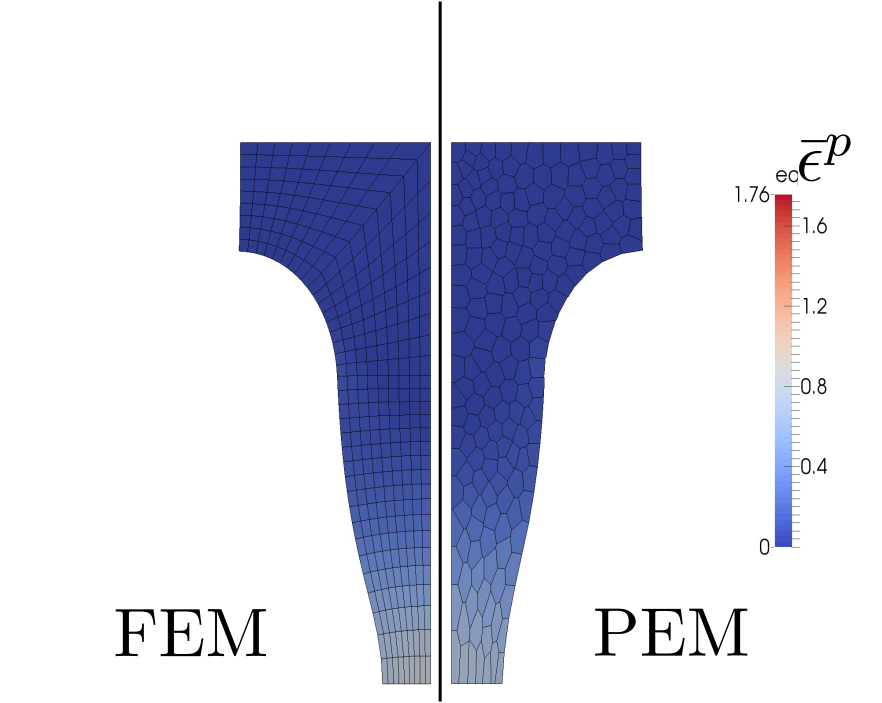
\includegraphics[width=3.0in]{figures/necking_eqps_1.pdf}
    			\caption{$t=0.5$ \label{fig:necking_eqps_1}}
    \end{subfigure}
    \begin{subfigure}[b]{0.49\linewidth}
            \centering
            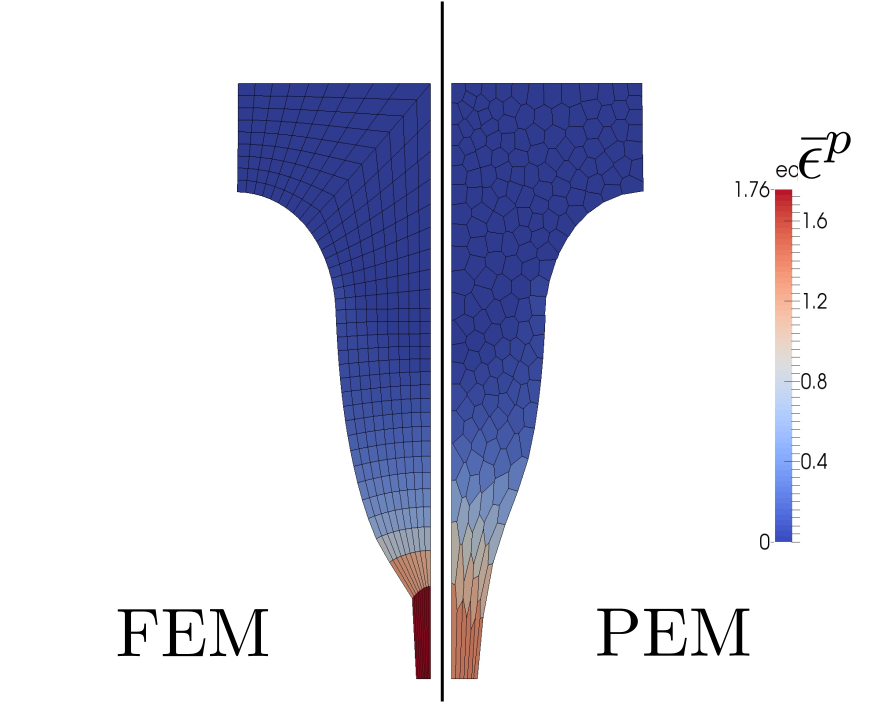
\includegraphics[width=3.0in]{figures/necking_eqps_2.pdf}
    			\caption{$t=0.75$ \label{fig:necking_eqps_2}}
    \end{subfigure}
	\begin{subfigure}[b]{0.49\linewidth}
            \centering
            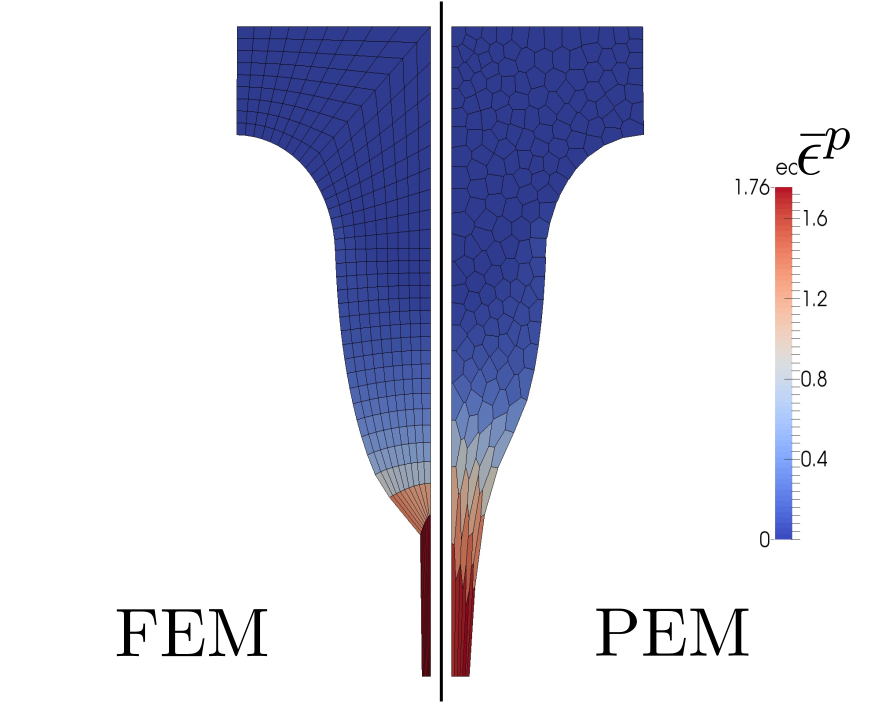
\includegraphics[width=3.0in]{figures/necking_eqps_3.pdf}
    			\caption{$t=1$ \label{fig:necking_eqps_3}}
    \end{subfigure}
    \caption{Comparison of necking behavior at various times during the analysis, depicting deformed shape, and values of equivalent plastic strain.}
\end{figure}

\subsection*{Taylor Bar Dynamic Impact}

\begin{figure}[!h]
  \centering
    \begin{subfigure}[b]{0.49\linewidth}
            \centering
            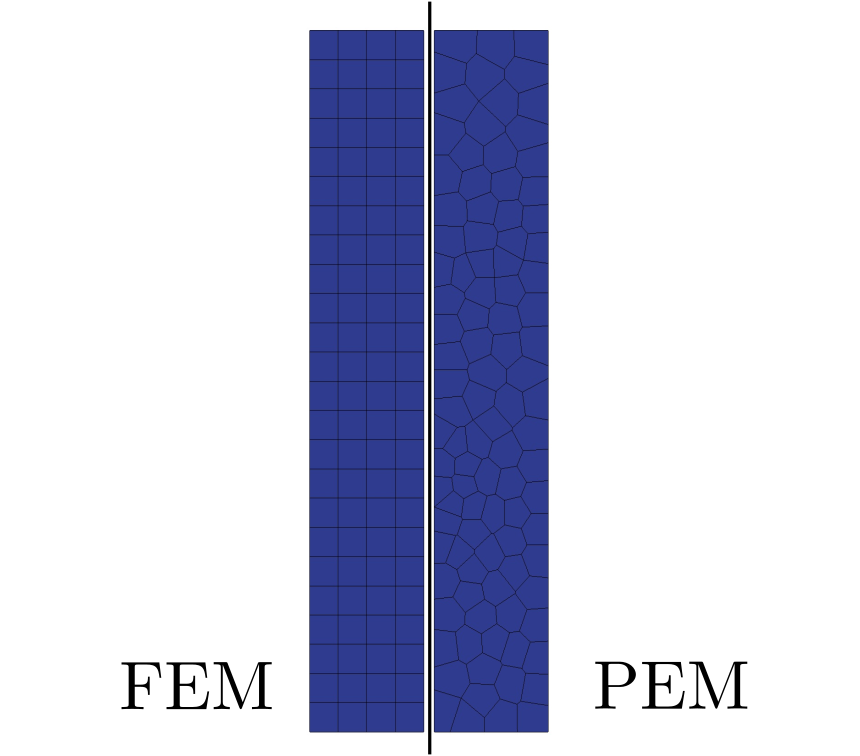
\includegraphics[width=3.0in]{figures/taylor_eqps_0.pdf}
    			\caption{$t=0.0$ \label{fig:taylor_eqps_0}}
    \end{subfigure}
	\begin{subfigure}[b]{0.49\linewidth}
            \centering
            \includegraphics[width=3.0in]{figures/taylor_eqps_1.pdf}
    			\caption{$t=1.0\times 10^{-6}$ \label{fig:taylor_eqps_1}}
    \end{subfigure} \caption{Comparison plot of the deformed shape and equivalent plastic strain $\bar{\epsilon}^p$ within the Taylor bar impact specimen.}
  \label{fig:taylor_eqps}
\end{figure}